
\chapter{Method}\label{chap:method}



%***********************************************************************************************
This chapter describes the methodological approach used to design, implement, and validate the proposed distributed acoustic measurement system. The methods are derived directly from the functional and non-functional requirements introduced in Chapter~\ref{Requierements}, with particular emphasis on timing determinism, wireless range, and audio acquisition performance.

The work follows an engineering-driven methodology. First, a system architecture is defined to separate time-critical audio processing from wireless communication and synchronization tasks. Second, the main design decisions are implemented and documented at the subsystem level, covering the computational core, the audio acquisition chain, the \acrshort{rf} communication, and the synchronization firmware. Finally, the proposed design is evaluated through targeted experiments that directly map to the system requirements.

The experimental validation focuses on three key aspects: wireless communication range in non-line-of-sight environments, microsecond-level synchronization response time of the wireless communication, and audio signal fidelity for impulse-response measurements. The following sections describe these activities and motivate the corresponding
design choices.

\section{System Architecture Overview} \label{sec:system_architecture_overview}

The system was designed with a heterogeneous, modular node architecture. The main objective of this architecture is to separate functions with different timing, noise, power, and communication requirements into dedicated subsystems. This avoids concentrating all tasks on a single general-purpose platform and allows each part of the node to be designed according to its specific constraints.

The architecture is organized around five main hardware blocks: the real-time audio subsystem, the \acrshort{rf} and synchronization subsystem, the analog front-end subsystem, the power subsystem, and the battery pack with protection circuitry. The audio subsystem handles playback and recording, while the \acrshort{rf} subsystem handles wireless communication and synchronization timing. The analog front end conditions the microphone input signal before digitization, and the power subsystem generates the regulated voltage rails required by the digital, analog, audio, and high-voltage sections of the node.

This partitioning was selected because the main subsystems impose several requirements. Audio acquisition requires stable sampling, predictable triggering, and low-noise analog operation. Wireless communication requires long-range packet exchange and accurate timing of radio events. The analog front end requires a clean interface between the measurement microphone and the audio subsystem, while the power subsystem must support both low-power operation and short high-current demands. By separating these functions, each subsystem can be developed and validated independently before full-system integration.

A dedicated interconnection stage routes the signals exchanged between subsystems. These signals include synchronization triggers, mode-selection lines, conditioned signals, and regulated power rails. Time-critical synchronization events are propagated through hardware GPIO signals instead of relying on software messages between processors. This allows the \acrshort{rf} subsystem to trigger the audio subsystem with bounded, deterministic, and repeatable latency, while keeping the communication logic separate from the audio acquisition path.

At the node level, the architecture supports different operating roles. A node can operate as a source, a receiver, or a combined source-receiver depending on the measurement configuration. Source operation requires controlled playback of the excitation signal, receiver operation requires synchronized acquisition of the acoustic response, and combined operation requires simultaneous playback and recording. This flexibility is important because the same hardware architecture can support different experimental setups without changing the basic synchronization concept.

At the network level, the system follows a master-slave star topology in the 868~MHz ISM band. The master node initiates synchronization and communication events, while the slave nodes receive \acrshort{rf} messages and execute time-aligned actions based on the received commands. This topology was selected because it provides a clear timing reference, simplifies protocol design, and makes synchronization behavior easier to validate experimentally.

The modular architecture also defines the validation strategy used in this work. The wireless subsystem can be evaluated through range and timing tests, the audio subsystem through playback and acquisition tests, the analog front end through signal-conditioning and microphone-interface tests, and the power subsystem through consumption and autonomy measurements. The complete system can then be validated by integrating these subsystems and verifying that synchronized acoustic measurements can be executed reliably.


\section{Computational and Firmware Architecture}

The computational architecture was defined from the requirements of the distributed measurement system. The system requires audio playback and recording, wireless communication, timestamping, synchronization triggers, local storage, and power-state control. These functions have different timing constraints, so they are not assigned to a single processor unit. Instead, the node uses dedicated  controllers for the audio and \acrshort{rf} synchronization subsystems.

One subsystem is dedicated to audio playback, acquisition, and local audio-data handling, while the other controller is dedicated to wireless communication and synchronization. This partitioning follows the system architecture described in Section~\ref{sec:system_architecture_overview}, where audio processing and \acrshort{rf}-based synchronization are treated as separate functional domains.


\subsection{Microcontroller Selection and Controller Partitioning}

A microcontroller-based architecture was selected because the system requires a predictable response to hardware events. In particular, synchronization events must be detected and converted into local actions with bounded latency. This is difficult to guarantee on a general-purpose processor running a non-real-time operating system, where interrupts, drivers, background processes, and scheduling can introduce additional jitter \cite{ALBERTOS2005203}.

Microcontrollers provide direct access to peripherals, hardware timers, interrupt controllers, DMA engines, and GPIO lines. This makes them suitable for event-driven synchronization and low-level control of audio and \acrshort{rf} interfaces. Therefore, the design prioritizes interrupt latency, timer resolution, peripheral control, and repeatable execution over general computational throughput.

The use of two controllers was selected to avoid assigning all time-critical and peripheral-intensive operations to a single processing unit. Audio acquisition requires stable digital audio interfaces, codec control, buffer management, and access to local storage. In contrast, the synchronization subsystem requires precise handling of radio events, packet timing, and hardware trigger signals. Keeping these functions on separate controllers reduces coupling between continuous audio streaming and wireless communication.

The audio controller is implemented using the STM32H735G-DK Discovery kit, which integrates an STM32H735IGK6 microcontroller, as shown in Figure \ref{fig:st_boa}. The STM32H7 family is based on the ARM Cortex-M7 core; the specific device used here provides 1 Mbyte of flash memory and 564 Kbytes of SRAM. This platform was selected because it offers sufficient processing capability for real-time audio handling while maintaining deterministic peripheral control. In particular, it integrates dedicated audio interfaces, DMA controllers, large on-chip memory, and external memory interfaces, which together simplify continuous audio streaming and buffering. These features enable audio acquisition and playback with limited processor intervention, reducing the risk of sample loss during long measurements.

\begin{figure}[h!]
    \centering
    \includegraphics[width=0.7\linewidth]{figures/st_board.png}
    \caption{ STM32H735G-DK Discover Kit evaluation board top view}
    \label{fig:st_boa}
\end{figure}

The board includes a comprehensive set of peripherals that support the evaluation of multiple functions and accelerate application development. These peripherals include USB OTG FS, Ethernet, a microSD\texttrademark{} card interface, USART, CAN FD, an SAI audio codec with stereo line input and output via audio jacks, a MEMS digital microphone, HyperRAM\texttrademark{}, Octo-SPI flash memory, and an RGB LCD with a capacitive touch panel. In addition, ARDUINO\textregistered{} Uno V3 connectors are provided, which simplify the integration of extension shields or daughterboards tailored to specific applications.

The WM8994 codec is embedded on the evaluation board and was chosen for its direct compatibility with the digital audio peripherals available on the STM32H7 platform. Additionally, the presence of the microSD\texttrademark{} card interface was convenient, as one of the project requirements was local audio recording. Together, the microcontroller and codec form a complete audio subsystem with sufficient performance margin for the required sampling rates and storage operations. The rationale for the codec selection is discussed in more detail in Section~\ref{sec:codec_selection}.

The \acrshort{rf} and synchronization controller is based on the Texas Instruments \linebreak CC1352Px wireless microcontroller shown in Figure \ref{fig:ccp}. This device was selected because the synchronization method depends on precise handling of radio events and on a tight interaction between the radio subsystem and the application firmware. The CC1352Px integrates an application processor together with a dedicated radio core, which manages low-level \acrshort{rf} operation and reports relevant events to the application through driver callbacks \cite{ti_cc1352px_ds}. %This allows the application firmware to react to packet transmission and reception events without managing the physical-layer radio operation directly.
\begin{figure}[h]
    \centering
    \includegraphics[width=0.9\linewidth]{figures/ccp.png}
    \caption{Texas instruments launchpad CC1352Px.}
    \label{fig:ccp}
\end{figure}

This architecture is preferable to using a general-purpose microcontroller with an external radio transceiver, since it avoids an additional communication interface between the processor and the radio device. As a result, packet handling, radio timing, and synchronization logic can be implemented within the same wireless microcontroller platform, simplifying the timing path and reducing integration complexity. The internal organization of the CC1352Px is shown in Figure~\ref{fig:cc1352px_rf_architecture}. The application MCU executes the synchronization logic and interacts with the RF driver API, while the RF core handles radio scheduling, physical-layer operation, and command execution. Communication between both parts is performed through RF commands and callbacks.

\begin{figure}[h]
    \centering
    \includegraphics[width=0.43\linewidth]{figures/cc1352px_rf_architecture.png}
    \caption{Internal organization of the CC1352Px \acrshort{rf} subsystem. The application MCU executes the synchronization logic and controls the RF driver. The RF core handles radio scheduling, physical-layer operation, and command execution.}
    \label{fig:cc1352px_rf_architecture}
\end{figure}

The CC1352Px architecture is also relevant for the timing requirements and the synchronization protocol. The application firmware runs on a 48~MHz Arm Cortex-M4F processor, which means approximately 1 clock cycle every 20.833~ns, and a dedicated Arm Cortex-M0 radio controller handles low-level \acrshort{rf} commands, radio scheduling, and physical-layer operation \cite{ti_cc1352px_ds}. This architecture allows synchronization algorithms to run on the main processor while radio scheduling, packet transmission, and reception timing remain tightly coupled to the hardware, providing a suitable timing interface for the event-based synchronization method. 

The resulting controller partitioning is summarized in Table~\ref{tab:controller_partitioning}. The selected devices were not chosen solely because they satisfy the functional requirements, but because their peripheral sets, timing characteristics, and architectural features align with the two critical tasks of the system: continuous audio acquisition and deterministic wireless synchronization. Using specialized controllers for each domain reduces implementation complexity and minimizes interference between audio processing and synchronization activities.

\begin{table}[h]
    \centering
    \caption{Controller partitioning in the measurement node.}
    \label{tab:controller_partitioning}
    \begin{tabular}{|p{0.27\linewidth}|p{0.28\linewidth}|p{0.35\linewidth}|}
        \hline
        \textbf{Subsystem} & \textbf{Controller} & \textbf{Main responsibilities} \\
        \hline
        Audio subsystem & STM32H7 + WM8994 & Audio playback, audio acquisition, codec control, buffer handling, and local audio-data storage. \\
        \hline
        \acrshort{rf} synchronization subsystem & CC1352Px & Sub-GHz communication, packet handling, radio timing, synchronization logic, and hardware trigger generation. \\
        \hline
    \end{tabular}
\end{table}

Figure~\ref{fig:computational_partitioning} summarizes the computational partitioning of the node. The audio and \acrshort{rf} controllers exchange only a limited set of hardware-level signals, such as trigger and mode-selection lines. This interface keeps the interaction between both domains simple and makes the timing path easier to analyze.

\begin{figure}[h]
    \centering
    \includegraphics[width=1\linewidth]{figures/computational_partitioning.png}
    \caption{Computational partitioning of the measurement node. STM32H 7- WM8994 audio subsystem and CC1352Px synchronization \acrshort{rf} subsystem.}
    \label{fig:computational_partitioning}
\end{figure}

%\subsection{Audio Controller and Processing Chain}

%\textcolor{red}{{I dont think describing twice this part is necessary}The audio controller is responsible for the real-time playback and acquisition path used during impulse-response measurements. The selected STM32H7 platform provides direct access to timers, GPIO interrupts, DMA transfers, serial audio interfaces, and local memory regions, which are required for deterministic audio operation. The WM8994 codec provides the analog-to-digital and digital-to-analog conversion stages used by the prototype.

%The audio path is organized around three main operations: codec configuration, audio streaming, and local data handling. Codec configuration is performed through a low-rate control interface, while audio samples are transported through the digital audio interface. This separation is useful because control transactions and continuous audio sample transport have different timing requirements.

%The audio firmware must support different operating modes. In playback mode, the excitation signal is reproduced through the output path. In recording mode, the acoustic response is acquired and stored. In full-duplex mode, playback and recording occur simultaneously. The need for these modes follows from the measurement configurations described in the background chapter, where nodes may operate as sources, receivers, or combined source-receiver units.

%For local recording, audio data must be moved from the acquisition interface to memory and then to storage without interrupting the audio stream. This motivates the use of buffered transfers and task-level separation between acquisition and file handling. In the current implementation, the audio subsystem also uses FreeRTOS to organize these activities into tasks while keeping time-critical audio operations tied to hardware events and peripheral transfers.

\subsection{RF Controller and Radio Processing Core}

The \acrshort{rf} controller provides the wireless communication and synchronization interface of the node. It is implemented using the CC1352Px platform because the application firmware can build packets, control the synchronization state, and interact with the rest of the node, while the radio core handles the lower-level radio operation \cite{ti_cc1352px_ds}.

In this architecture, the \acrshort{rf} controller is not used for continuous audio-data streaming. Its role is to exchange short control and synchronization packets, estimate timing information, and generate hardware-level synchronization outputs. This reduces radio channel occupancy and keeps the wireless link focused on timing coordination rather than high-throughput data transfer.

The detailed packet exchange, ranging procedure, one-way-time estimation, and synchronization scheduling are described in the following \acrshort{rf} synchronization method section. The \acrshort{rf} controller is treated as a dedicated synchronization processor rather than as a general communication peripheral attached to the audio controller.

\subsection{FreeRTOS Execution Model}
\label{sec:freertos_model}
FreeRTOS is used on both embedded controllers to provide a structured firmware execution model based on tasks, priorities, and synchronization mechanisms \cite{FreeRTOSOverview, FreeRTOSScheduling}. The firmware is mainly event-driven, so tasks are not intended to run continuously while waiting for work. Instead, they remain blocked until a relevant event occurs, such as an external trigger, a timer expiration, the completion of a peripheral transfer, or the availability of data in a buffer. This avoids unnecessary polling and makes the execution flow easier to analyze.

Interrupts are used to connect hardware events to the task-level firmware. When a hardware event occurs, the corresponding interrupt service routine is kept short and only performs the minimum operation needed to notify the firmware. The complete application logic is therefore not executed inside the interrupt itself. Instead, the interrupt releases or notifies the corresponding task using a FreeRTOS synchronization mechanism, such as a semaphore or task notification. The task then performs the required operation in a controlled context \cite{FreeRTOSTaskNotifications}.

Task priorities are used to define which activity is executed first when several tasks are ready at the same time. Time-critical tasks are assigned higher priority than non-critical tasks, so that synchronization, audio control, and data movement can be handled before debug or background operations. This does not replace hardware timers, DMA, or peripheral-level timing, but it reduces the possibility that low-priority firmware activity interferes with measurement-related actions \cite{FreeRTOSScheduling}.

FreeRTOS synchronization mechanisms are used to coordinate tasks and shared resources. Mutexes are used when a shared resource must only be accessed by one task at a time, while semaphores and task notifications are used to signal events between interrupts, callbacks, and tasks. Queues are used when information, commands, or buffer references must be passed between tasks without directly sharing memory \cite{FreeRTOSMutexes, FreeRTOSQueues, FreeRTOSTaskNotifications}.

This execution model is applied to both the audio and \acrshort{rf} controllers. In the audio subsystem, tasks are organized around audio control, buffer handling, storage, and trigger response. In the \acrshort{rf} subsystem, tasks are organized around communication requests, packet handling, and synchronization control. Events define when time-critical actions start, while FreeRTOS provides the task structure used to execute the corresponding firmware operations.


\section{RF Synchronization}
\label{sec:rf_synchronization}

This section describes the \acrshort{rf} synchronization method used to coordinate measurement actions between distributed nodes. The objective of the method is to allow spatially separated nodes to execute playback or recording actions with bounded timing error and without wired trigger lines.

The synchronization method is divided in two stages. First, a ranging stage is used to estimate the timing relation between the master and the slave nodes. Then, a synchronization stage uses this timing information to schedule local hardware-triggered actions. The system relies on packet events, local timers, and GPIO trigger signals to execute the measurement action at the required time.

The details of the packet structure, ranging calculation, scheduling procedure, and multi-node extension are described in the following subsections.

\subsection{RF Configuration and Protocol Basis}

The \acrshort{rf} subsystem was configured to operate in the 868~MHz band using a proprietary GFSK-based mode supported by the CC1352Px platform. This configuration was selected according to two main system requirements: communication over long distances in partially obstructed environments and bounded timing behavior for synchronization events.

The use of the 868~MHz band is aligned with the range requirement of the system. Compared with 2.4~GHz alternatives, sub-GHz operation generally provides better propagation and penetration in obstructed environments, which is relevant for outdoor or cluttered measurement scenarios. In addition, the system must operate without relying on external communication infrastructure, so cellular-based solutions such as NB-IoT are not suitable for the intended deployment.

The selected protocol also requires bidirectional and low-latency packet exchange. The master must transmit short control packets, receive responses from the slaves, and use these radio events as timing references. For this reason, technologies with long packet time-on-air or limited downlink capability are not appropriate for the synchronization task. LoRa-based communication can provide long range, but its lower data rates, longer time-on-air, and ambiguity in defining the exact packet-arrival instant reduce its suitability as a deterministic timing reference \cite{raza2017rf, prando2019rf}.

A proprietary GFSK-based mode was selected because it provides shorter packet transactions and more clearly defined packet transmission and reception events than chirp-based spread-spectrum modes. This is important because the synchronization method depends on repeatable packet events. The reduced time-on-air also lowers channel occupancy, which is useful when the master must communicate sequentially with several slave nodes.

\subsection{Master--Slave Star Topology}

The \acrshort{rf} synchronization protocol is organized as a master--slave star topology. In this structure, a single node operates as the master and coordinates the synchronization process, while the remaining nodes operate as slaves. The master is responsible for initiating the \acrshort{rf} transactions, selecting the target node, collecting timing information during the ranging stage, and starting the synchronization stage. 

As shown in Figure~\ref{fig:rf_star_topology}, the architecture is conceived for one master node and up to five slave nodes. The arrows indicate the bidirectional communication. The master sends commands and synchronization packets, while the slaves return responses during the ranging and synchronization procedures. 

\pagebreak
\begin{figure}[h]
    \centering
    \includegraphics[width=1\linewidth]{figures/rf_star_topology.png}
    \caption{Master--slave star topology used for \acrshort{rf} synchronization.}
    \label{fig:rf_star_topology}
\end{figure}

Each slave node is assigned a unique identifier. This allows the master to address nodes individually and control which node must respond at a given moment. On the slave side, packets are processed if the target identifier matches the local node identifier or if the packet corresponds to a broadcast command. This avoids unnecessary responses and keeps the communication channel under the control of the master. The use of a master--slave topology simplifies the synchronization model as the slaves do not initiate timing exchanges on their own. Instead, they react to valid packets received from the master. 

\pagebreak
\subsection{Packet Structure}

The \acrshort{rf} protocol uses a fixed-length payload of 10 bytes. The packet is kept short because it is only used for control and synchronization. Each packet contains the information required to identify the target node, identify the sender, associate requests with responses, encode auxiliary actions, and transmit timing information for the synchronization stage.

The first two bytes define the addressing information. Byte~0 contains the target identifier and Byte~1 contains the source identifier. In packets transmitted by the master, the target identifier corresponds to the selected slave node. In echo responses transmitted by a slave, the target identifier is set to the master identifier. This structure allows both sides to verify that the received packet belongs to the expected transaction.

Bytes~2 and~3 contain the sequence number. The sequence number is incremented by the master and copied by the slave in the echo response. This allows the master to associate a received echo with the packet that generated it, avoiding the use of outdated or unrelated responses during the ranging and synchronization stages.

Byte~4 is reserved as an auxiliary field. This field can be used to carry operation-specific information without modifying the rest of the packet format. Byte~5 is used as the synchronization flag. A value of \texttt{0x00} corresponds to the ranging stage, while \texttt{0xFF} indicates that the packet is a synchronization command. Bytes~6 to~9 contain a 32-bit delay value in microseconds. During the synchronization stage, this value is used by the slave to configure a local one-shot timer.

Figure~\ref{fig:rf_packet_structure} summarizes the packet format used by the protocol.

\begin{figure}[h]
    \centering
    \includegraphics[width=0.95\linewidth]{figures/rf_packet_structure.png}
    \caption{Fixed-length \acrshort{rf} communication payload.}
    \label{fig:rf_packet_structure}
\end{figure}



\subsection{Synchronization Protocol}

The synchronization protocol is based on a master-controlled request--response transaction. The master initiates every transaction by transmitting an addressed packet to a slave node. The slave node transmits only after receiving and validating a packet from the master. This avoids simultaneous responses and keeps the half-duplex \acrshort{rf} channel under the control of the master.

Figure~\ref{fig:sync_protocol_transaction} shows the base transaction used by the protocol. The master schedules an \acrshort{rf} transmission at time $t_{TX}$. When the packet is received by the slave, the slave verifies the target identifier, source identifier, and sequence number. If the packet is valid, the slave returns an echo response after a fixed echo delay. The master receives this response at time $t_{RX}$ and uses the elapsed time between transmission and reception to obtain the timing information required by the protocol.

\begin{figure}[t]
	\centering
	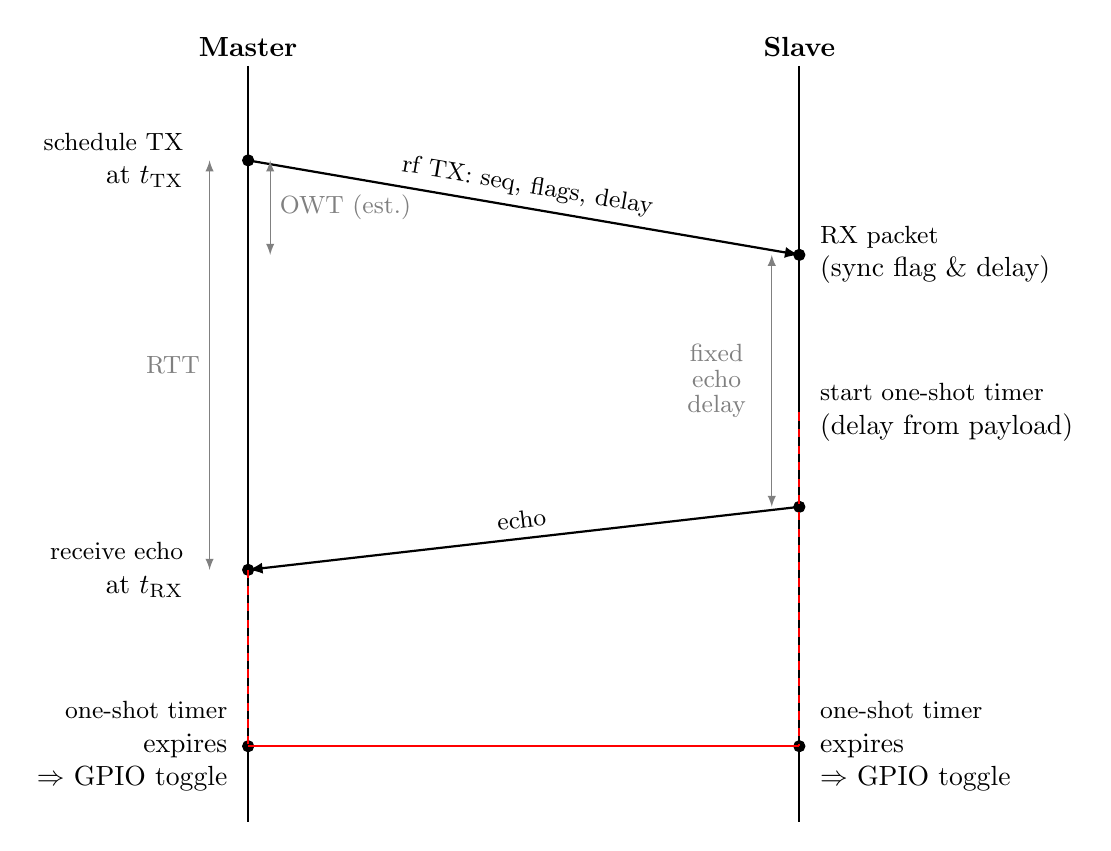
\begin{tikzpicture}[x=0.7cm,y=0.8cm,>=latex]  
		
		% Lifelines 
		\draw[thick] (2,0) -- (2,-12);
		\draw[thick] (12,0) -- (12,-12);
		\node[above] at (2,0) {\textbf{Master}};
		\node[above] at (12,0) {\textbf{Slave}};
		
		% Master events
		\node[anchor=east,align=right] at (1,-1.5) {\small schedule TX\\ at $t_\mathrm{TX}$};
		\draw[fill=black] (2,-1.5) circle (2pt);
		
		\node[anchor=east,align=right] at (1,-8) {\small receive echo\\ at $t_\mathrm{RX}$};
		\draw[fill=black] (2,-8.0) circle (2pt);
		
		\node[anchor=east,align=right] at (1.8,-10.8) {\small one-shot timer\\ expires\\$\Rightarrow$ GPIO toggle};
		\draw[fill=black] (2,-10.8) circle (2pt);
		
		% Slave events
		\node[anchor=west,align=left] at (12.2,-3.0) {\small RX packet\\(sync flag \& delay)};
		\draw[fill=black] (12,-3.0) circle (2pt);
		
		\node[anchor=west,align=left] at (12.2,-5.5) {\small start one-shot timer\\(delay from payload)};
		
		\node[anchor=west,align=left] at (12.2,-10.8) {\small one-shot timer\\ expires\\$\Rightarrow$ GPIO toggle};
		\draw[fill=black] (12,-10.8) circle (2pt);
		
		% Message: Master TX -> Slave RX
		\draw[->,thick] (2,-1.5) -- (12,-3.0)
		node[midway,above,sloped] {\small \acrshort{rf} TX: seq, flags, delay};
		
		% RTT and OWT measurements
		\draw[<->,gray] (1.3,-1.5) -- (1.3,-8.0) 
		node[midway,left,align=center] {\small RTT};
		
		\draw[<->,gray] (2.4,-1.5) -- (2.4,-3.0) 
		node[midway,right] {\small OWT (est.)};
		
		% Echo: Slave TX -> Master RX
		\draw[fill=black] (12,-7.0) circle (2pt);
		\draw[->,thick] (12,-7.0) -- (2,-8.0)
		node[midway,above,sloped] {\small echo};
		
		% echo delay annotation
		\node[gray,align=center] at (10.5,-5.0) {\small fixed\\[-1mm]\small echo\\[-1mm]\small delay};
		\draw[<->,gray] (11.5,-3.0) -- (11.5,-7.0);
		
		% Timer scheduling lines (dashed) - RED
		\draw[dashed,red,thick] (12,-5.5) -- (12,-10.8);
		\draw[dashed,red,thick] (2,-8.0) -- (2,-10.8);
		
		% Horizontal line connecting the timer triggers - RED
		\draw[red,thick] (2,-10.8) -- (12,-10.8);
		
	\end{tikzpicture}
	\caption{Timing diagram of the two-node master--slave synchronization procedure.
	The slave schedules its action directly from the synchronization packet, while the
	master schedules its local action relative to the same \acrshort{rf} transaction and the
	measured timing.}
    \label{fig:sync_protocol_transaction}
\end{figure}

The synchronization flag defines how the received packet is interpreted. When the flag is inactive, the transaction is used in ranging mode. In this mode, the slave only returns the echo response, no measurement trigger is generated and the slave is marked as reachable. The master uses the measured round-trip time, corrected by the fixed echo delay, to estimate the one-way time between the master and the addressed slave.

Figure~\ref{fig:ranging_mode_timeline} shows how the ranging transaction is applied over time. After every master's message is sent, the slaves keep a small fixed delay before sending the echo replies to give enough processing time. Nevertheless, if the master's waiting time exceeds a configurable timeout, the transaction is considered unsuccessful. Then the master will retry a configurable number of attempts and then continue with the next node. This prevents one missing response from blocking the complete ranging procedure.

\begin{figure}[h]
    \centering
    \includegraphics[width=1.1\linewidth]{figures/ranging_mode_timeline.pdf}
    \caption{Ranging-mode execution of the synchronization protocol. The master queries slave nodes sequentially and uses the echo responses to estimate the one-way time.}
    \label{fig:ranging_mode_timeline}
\end{figure}

When the synchronization flag is active, the transaction is used in synchronization mode, where only reachable slaves are addressed. The slaves still only echo after receiving and validating the packet. Then master uses the response to confirm that the synchronization command was received. If the response is not received before the timeout expires, the master will not retry but continue with the remaining nodes. This is done to avoid recalculation and re--sending messages to all nodes.

Figure~\ref{fig:synchronization_mode_timeline} shows the synchronization-mode execution. The master sends synchronization commands sequentially, using the timing information obtained during ranging. Each slave starts its local timer after receiving its command, so the final trigger instant is defined locally by hardware timers rather than by continuous wireless communication. This reduces the dependency on software execution time during the final measurement trigger.

\begin{figure}[h]
    \centering
    \includegraphics[width=1\linewidth]{figures/synchronization_mode_timeline.pdf}
    \caption{Synchronization-mode execution of the protocol. Each addressed slave receives a timer delay and schedules its local one-shot timer.}
    \label{fig:synchronization_mode_timeline}
\end{figure}

The same packet format is therefore used for both stages. In ranging mode, the packet exchange provides timing information. In synchronization mode, the packet carries the timing command used to schedule the hardware trigger. The detailed calculation of the one-way time and the firmware implementation of the algorithm are described in the following subsections.


\subsection{One-Way Time Estimation}

The ranging stage estimates the one-way time between the master and each reachable slave. This value is obtained from the request--response transaction shown in Figure~\ref{fig:sync_protocol_transaction}. The master records the time at which the packet transmission is scheduled, $t_{TX}$, and the time at which the echo response is received, $t_{RX}$.

The measured round-trip interval is therefore

\begin{equation}
    t_{RTT,meas} = t_{RX} - t_{TX}.
\end{equation}

This interval includes the propagation and radio latency in both directions, as well as the fixed delay introduced by the slave before transmitting the echo response. Since this echo delay is known, it is subtracted from the measured round-trip interval:

\begin{equation}
    t_{RTT} = t_{RTT,meas} - t_{echo}.
\end{equation}

Assuming that the forward and return paths have approximately the same delay, the one-way time is estimated as

\begin{equation}
    t_{OWT} = \frac{t_{RTT}}{2}.
\end{equation}

Substituting the previous expression gives

\begin{equation}
    t_{OWT} = \frac{t_{RX} - t_{TX} - t_{echo}}{2}.
\end{equation}


The estimated one-way time includes the physical propagation delay of the \acrshort{rf} signal and the radio-related transmission and reception latencies. The propagation component can be approximated as

\begin{equation}
    t_{prop} = \frac{d}{c},
\end{equation}

where $d$ is the distance between nodes and $c \approx 3 \times 10^8~\mathrm{m/s}$ is the speed of electromagnetic propagation in air. This gives approximately $0.33~\mu s$ per 100~m, or $3.33~\mu s$ for a 1~km link.

In addition, the measured one-way time also includes radio transmission and reception latency, so the ranging procedure estimates the effective timing delay of the complete \acrshort{rf} transaction rather than only the physical propagation time.

The estimated one-way time is stored independently for each slave node. During the synchronization stage, this value is used to compensate for the delay between the master transmission and the slave reception. Therefore, each slave can receive a different timer-delay value, depending on its estimated timing relation with the master.

To improve the stability of the OWT estimate, the ranging transaction is executed three times for each node before every synchronization stage. The three measurements are averaged, and the resulting value is used in the synchronization-delay calculation.
 
The estimation does not require continuous clock synchronization between nodes. All timing measurements are made by the master using its local \acrshort{rf} timer, while the slave only introduces a fixed echo delay and returns the received sequence number. This keeps the ranging procedure simple and avoids the need to exchange absolute timestamps between nodes.



\subsection{Synchronization Delay Calculation}

After the ranging stage, the master defines a common target instant for the synchronization event. This target must be sufficiently far in the future to allow the master to send the synchronization command to every reachable slave and receive the corresponding echo responses.

For each slave $i$, the synchronization packet contains a timer delay calculated from the remaining time to the target instant and the estimated one-way time:

\begin{equation}
    t_{\mathrm{delay},i}
    =
    t_{\mathrm{target}}
    -
    t_{\mathrm{TX},i}
    -
    t_{\mathrm{OWT},i},
\end{equation}

where $t_{\mathrm{target}}$ is the common synchronization instant, $t_{\mathrm{TX},i}$ is the scheduled transmission time of the packet addressed to slave $i$, and $t_{\mathrm{OWT},i}$ is the one-way time estimated during ranging.

When the packet reaches the slave, the remaining delay to the target instant is therefore approximately

\begin{equation}
    t_{\mathrm{remaining},i}
    =
    t_{\mathrm{delay},i}
    -
    t_{\mathrm{fw},i},
\end{equation}

where $t_{\mathrm{fw},i}$ represents the local firmware latency between packet reception and completion of the timer configuration. This correction is applied before loading the one-shot timer.

The master uses the same target instant for its local trigger. After receiving the echo response, it calculates the remaining interval as

\begin{equation}
    t_{\mathrm{remaining,M}}
    =
    t_{\mathrm{target}}
    -
    t_{\mathrm{current}}
    -
    t_{\mathrm{fw,M}},
\end{equation}

where $t_{\mathrm{current}}$ is the master time when the local timer is prepared and $t_{\mathrm{fw,M}}$ is the measured master-side firmware latency.

As a result, the master and all addressed slaves use independent local timers but reference the same target instant. Differences in RF delay are compensated using the node-specific OWT estimates, while differences in local firmware execution are compensated using measured latency constants.


\subsection{Firmware Implementation and Timing Compensation}

The firmware implementation is event-driven and uses RF callbacks, GPIO interrupts, FreeRTOS tasks, and one-shot timers. The protocol execution is assigned to a high-priority RF task, while diagnostic communication is handled by a lower-priority UART task. Table~\ref{tab:sync_resources} summarizes the main resources used by the synchronization firmware.

\begin{table}[h]
    \centering
    \caption{Resources used by the synchronization firmware.}
    \label{tab:sync_resources}
    \begin{tabular}{|p{0.22\linewidth}|p{0.28\linewidth}|p{0.40\linewidth}|}
        \hline
        \textbf{Resource} & \textbf{Configuration} & \textbf{Function} \\
        \hline
        RF subsystem &
        Proprietary 868~MHz GFSK mode with address filtering &
        Executes packet transmission and reception and reports RF events to the application firmware. \\
        \hline
        RF timer &
        4~MHz timing source with $0.25~\mu s$ resolution &
        Schedules RF transmissions and timestamps request--response transactions. \\
        \hline
        One-shot timer &
        Single-expiration callback &
        Generates the final synchronized action locally at each node. \\
        \hline
        GPIO inputs &
        Internal pull-up and falling-edge detection &
        Read external control signals and initiate the synchronization procedure through an interrupt. \\
        \hline
        GPIO outputs &
        Initially inactive digital outputs &
        Generate synchronization, microphone-control, and speaker-control pulses. \\
        \hline
        FreeRTOS tasks &
        Priority-based preemptive execution &
        Separate the timing-critical RF procedure from UART and background operations. \\
        \hline
        UART interface &
        Buffered output from a lower-priority task &
        Reports status and timing measurements without blocking the critical execution path. \\
        \hline
    \end{tabular}
\end{table}

The synchronization procedure is initiated by a falling-edge GPIO interrupt. The interrupt service routine is kept short and only notifies the task responsible for launching the RF procedure. The protocol is then executed by the high-priority RF task. While this task remains ready, lower-priority tasks, including UART communication, cannot preempt it. The critical execution path therefore operates with minimal interference from the operating system, although FreeRTOS remains active. Interrupt-level events, including RF events and timer expiration, can still preempt task execution.

Figure~\ref{fig:rf_firmware_execution} summarizes the execution path and the priority separation used by the firmware.

\begin{figure}[!h]
    \centering
    \includegraphics[width=0.95\linewidth]{figures/rf_firmware_execution.png}
    \caption{Interrupt-driven execution path and task-priority separation used by the synchronization firmware.}
    \label{fig:rf_firmware_execution}
\end{figure}

RF operations are executed using scheduled commands and driver callbacks. On the master, the transmission instant is referenced to the RF timer, and the reception callback provides the timestamp associated with the echo response. On the slave, packet reception and echo transmission are linked through the RF command sequence, preserving the fixed response delay used by the OWT calculation.

The final trigger is generated by a local one-shot timer rather than by the RF task. Once the required delay is available, the firmware applies the corresponding correction, configures the timer period, and starts the timer. When the timer expires, its callback generates a short synchronization pulse and updates the microphone and speaker control outputs. This removes task scheduling from the final trigger instant.

UART activity is kept outside the critical path. Diagnostic messages and measured timing values are copied into a software buffer and transmitted later by the lower-priority UART task. Therefore, UART formatting and transmission do not delay RF processing or timer configuration.

The OWT estimation compensates for the delay observed through the RF transaction. However, it does not include the local instruction time between the availability of the calculated delay and the effective start of the one-shot timer. This interval includes delay processing, application of correction terms, timer-period configuration, and timer start.

The local firmware latency was measured using internal timestamps. As shown in Figure~\ref{fig:firmware_latency_measurement}, the first timestamp, $T_1$, corresponds to the reception of the echo response. The second timestamp, $T_2$, was recorded after the remaining delay had been processed and the local one-shot timer had been configured. The measured interval, $\Delta t = T_2 - T_1$, was stored in the UART buffer and printed later by the lower-priority UART task. This avoided introducing UART transmission into the timing-critical execution path.

\begin{figure}[!h]
    \centering
    \includegraphics[width=0.95\linewidth]{figures/firmware_latency_measurement.png}
    \caption{Measurement of the local firmware latency using internal timestamps and deferred UART output.}
    \label{fig:firmware_latency_measurement}
\end{figure}

The measurement was performed independently for the master and slave because both nodes follow different processing paths before starting their local timers. In each case, the measured interval begins when the relevant RF event is received and ends after the timer has been configured. On the slave, this includes reading the received delay, applying the compensation, and configuring the one-shot timer. On the master, it includes calculating the remaining delay after echo reception, applying the required corrections, and configuring the local timer. The resulting latency is then subtracted from the corresponding timer delay to compensate for the firmware execution time.

Finally, Table~\ref{tab:sync_timing_components} summarizes the main sources of delay that affect the synchronization process and indicates how each one is treated by the implementation. Some components, such as RF propagation and transceiver latency, are included in the measured OWT, while local firmware execution time must be compensated separately. The table also includes the RF timer resolution, since it defines the smallest interval that can be represented by the timing measurements and scheduled radio events.


\begin{table}[!h]
    \centering
    \caption{Timing considerations and compensation mechanisms.}
    \label{tab:sync_timing_components}
    \begin{tabular}{|p{0.31\linewidth}|p{0.21\linewidth}|p{0.38\linewidth}|}
        \hline
        \textbf{Component} & \textbf{Magnitude} & \textbf{Treatment} \\
        \hline
        RF propagation &
        $0.33~\mu s$/100~m &
        Included in the OWT estimate. \\
        \hline
        RF TX/RX latency &
        $10$--$100~\mu s$ &
        Partially included in the measured OWT. \\
        \hline
        Slave firmware latency &
        $\approx 33~\mu \pm 10~\mu s$ &
        Measured with internal timestamps and subtracted from the received timer delay. \\
        \hline
        Master firmware latency &
        $\approx 86~\mu \pm 10~\mu s$ &
        Measured with internal timestamps and included in the remaining-delay calculation. \\
        \hline
        RF timer resolution &
        $0.25~\mu s$ &
        Resolution of RF timestamps and scheduled commands. \\
        \hline
    \end{tabular}
\end{table}

On the slave, the measured execution latency is subtracted from the delay received in the synchronization packet before the one-shot timer is loaded. On the master, the measured latency is included in the calculation of the remaining delay after reception of the echo. Separate compensation values are required because packet handling and timer preparation follow different execution paths on the two node types.

The final synchronization instant is therefore determined by the measured RF timing, the OWT correction, the node-specific firmware-latency compensation, and the local one-shot timer. Lower-priority task execution and UART communication remain outside this timing-critical path.

\section{Audio Processing Subsystem}
\label{sec:audio_subsystem}
The audio processing subsystem is responsible for real-time acquisition and playback of the excitation and response signals during impulse-response measurements. It is implemented around an STM32H7 microcontroller interfaced with a WM8994 audio codec, which together provides the digital audio interface, codec control, and local handling of audio streams. The STM32H7 platform provides direct access to timers, GPIO interrupts, DMA transfers, serial audio interfaces, and local memory regions required for deterministic audio operation.

The audio path separates two operations with different timing requirements: codec configuration, performed through a low-rate control interface (\acrshort{i2c}), and continuous audio sample transport, carried over the digital audio interface (SAI). For local recording, audio data must be moved from the acquisition interface to memory, then to storage, without interrupting the audio stream, which motivates buffered transfers and task-level separation between acquisition and file handling.
 
The role of this subsystem in the synchronization architecture is to react to hardware trigger signals generated by the \acrshort{rf} subsystem. These trigger signals are connected to interrupt-capable GPIO inputs, so the audio microcontroller can start or stop time-critical audio operations without relying on high-level software communication between processors.


\subsection{Codec and Converter Selection Criteria}
\label{sec:codec_selection}
To determine the optimal audio hardware, a two-phase methodology was employed: first, a component-level analysis of audio codecs and converters commonly used in audio applications, followed by an integrated system evaluation of available embedded processing platforms.

A comparative evaluation of the available integrated circuits (\acrshort{ic}s) against the project's high-fidelity requirements used the following exclusion criteria: 
\begin{itemize}
    \item Signal-to-Noise Ratio (\acrshort{snr}): any codec with an SNR below 90dB was discarded as it would fail to provide the necessary noise floor separation for accurate \acrfull{ir} characterization.
    \item Sample Rate Support: the options that didn't support sample rates of at least 48kHz were excluded to ensure that the Nyquist Frequency covers test signals like an Exponential Sine Sweep that will be reproduced from 20 Hz to 20kHz.
    % CORRECTED
    \item Bit depth: codecs that offered 24-bit were preferred to provide extra headroom during the recording and post signal processing. Although the WM8994 supports 24-bit operation, the firmware was configured at 16 bits to match the STM32H7 SAI default slot width and to reduce the DMA transfer bandwidth, which is sufficient given the 81.1~dB SNR measured at the codec baseline (Section~\ref{sec:res_thd}).
    \item Channel architecture: a preference for architectures that support simultaneous multi-channel recording was made to facilitate future expansion of the microphone array system. 
\end{itemize}


\subsection{Tools and initial configuration}
\label{sec:audio_tools}

This Section describes the activities undertaken to configure the selected audio system to capture an input signal, and the rationale for the tools chosen at each step. The system was brought to a working state through an iterative diagnosis-and-correct process; the observed symptoms are presented alongside the corrections that resolved them.

\subsubsection{X-CUBE-AUDIO-KIT}

STMicroelectronics offers an expansion package called X-CUBE-AUDIO-KIT that provides an integrated platform for designing, implementing, and fine-tuning audio processing data flows across a supported series of STM32 microcontrollers, including the STM32H735, which is selected as the audio hardware for this project.

This package includes a tool called LiveTune, a graphical user interface accessible via an HTML5 browser, where users can design and fine-tune data flows in real time on STM32 devices. An audio dataflow is described as a set of elements connected by a multi-frame buffer. The tool uses several types of elements, each symbolized by a dedicated icon.

As shown in Figure~\ref{fig:x_cube_structure}, this package adds a framework and middleware layer above the standard STM device workflow. The AudioChain firmware enables the generic implementation of the audio data flows mentioned, allowing the construction of a variety of complex workflows. AudioChain processes input from audio buffers and sends output to buffers, making it independent of specific hardware and BSP code.

Users can also integrate and fine-tune custom algorithms within the AudioChain environment, executing them as part of the audio data flows. This expansion package is designed for key applications such as voice denoising for speech recognition, audio output enhancement, and sound generation, among other audio processing scenarios.

\begin{figure}[h!]
  \centering
  \includegraphics[width=\textwidth]{figures/X-CUBE-AUDIO-KIT_structur.png}
  \caption{X-CUBE-AUDIO-KIT framework structure}
  \label{fig:x_cube_structure}
\end{figure}

To verify that the hardware was not faulty, the tool was configured in a pass-through setup using the STM32 BSP libraries. In this configuration, an AudioChain Source element was routed to the hardware audio input, which was the evaluation board's line-in. For the output path, a Sink element was defined and mapped to the system's line-out. The pass-through block configuration is shown in Figure~\ref{fig:pass_th}.

\begin{figure}[h!]
  \centering
  \includegraphics[width=\textwidth]{figures/pass_th.png}
  \caption{Pass through blocks in LiveTuner environment}
  \label{fig:pass_th}
\end{figure}

The first validation test used the signal generator of a DSOX2002A XR1-class oscilloscope (70~MHz, 2 analog channels, with a built-in function/waveform generator). A sine wave with a $\sim100$~mV peak-to-peak amplitude at 440~Hz was generated and fed into the line-in, and the line-out was connected to the oscilloscope. The following test involved connecting a pair of headphones (Anker Soundcore Life Q30) to the line-out to hear the output. A 440~Hz sinusoidal tone (A440, or A4) was chosen to match the pitch detector used in the Tuner application for the second test; this frequency is important to test because it is an internationally recognized standard for musical pitch.

The last test used the algorithm elements responsible for processing blocks and tools, which are mainly used as visualizers. An FFT algorithm was used to obtain the spectral analysis of the input signal. Between audio tests, this tool was uploaded to the board to check for any damage and whether the output or input results were not as desired.

As mentioned in the description, LiveTuner is primarily oriented toward applications such as guitar effects or scenarios where an output is actively played back or an input is constantly received. Consequently, the audio stream is always active, which was not desired for this system. Once a task started playback, it was not possible to stop it cleanly, and due to the way the audio chains were configured, extracting the required data was not straightforward. In addition, the goal was not to generate a single tone, but to read and play back arbitrary excitation signals, which required reading from an SD card. Because the audio was always playing, it was inconvenient to trigger these tasks according to specific schedules. A more flexible environment was therefore needed to achieve the desired system behavior. For this reason, the implementation was migrated to use the Board Support Package (\acrshort{bsp}) audio driver directly, together with FreeRTOS.

\subsubsection{\acrshort{bsp} Audio Driver Configuration and Clock Synchronization}
\label{sec:bsp_config}

The advantage of the \acrshort{bsp} audio driver is that it can be integrated within a FreeRTOS real-time multitasking architecture. By utilizing the raw \acrshort{bsp} driver, the restrictive abstraction barriers found in the generic application templates provided by LiveTuner are removed, granting direct control over peripheral registers and DMA streams. This low-level access is critical for handling the precise timing constraints of high-fidelity acoustic processing. Additionally, by using FreeRTOS, it is possible to guarantee deterministic task scheduling, enabling the system to handle background communication with the wireless module without interrupting time-critical audio acquisition loops or causing buffer underruns. Details related to speaker output routing and amplifier class selection, which primarily modify the codec driver rather than the acquisition path, are discussed separately in Section~\ref{sec:speaker}.

In the initial development phase, the onboard audio codec WM8994 was evaluated at a target sampling rate of \SI{96}{\kHz}. Initial testing focused on independently validating the Digital-to-Analog Converter (\acrshort{dac}) and Analog-to-Digital Converter (\acrshort{adc}) drivers, by reproducing a mathematically generated Exponential Sine Sweep (\acrshort{ess}) through the \acrshort{dac} and attempting capture through the \acrshort{adc}. A systematic diagnostic approach was designed to isolate driver and clocking discrepancies.

The \acrshort{dac} driver operated successfully, reproducing the \acrshort{ess} without audible artifacts, thereby confirming stable \SI{96}{\kHz} playback. The \acrshort{adc} driver, however, failed during these high-sample-rate configurations. The diagnostic confirmed that this behavior is a fundamental hardware limitation of the WM8994: while the \acrshort{dac} path (AIF1 input) supports operation at 88.2~kHz and 96~kHz, the \acrshort{adc} path (AIF1 output) is architecturally restricted to lower sampling rates. As stated in the datasheet, `88.2 kHz and 96 kHz modes are supported for AIF1 input (\acrshort{dac} playback) only.' Consequently, the final system configuration was set at a unified sampling rate of 48~kHz for both playback and recording.

\subsubsection{Diagnostic Procedure and Driver Modifications}
\label{sec:driver_mods}

After the isolated tests, both the input and output paths were integrated into a pass-through configuration to validate that the reference vendor-supplied BSP library had been adapted correctly. It is important to note that the default BSP framework is natively optimized for MEMS microphone arrays operating at standard \SI{44.1}{\kHz} or \SI{48}{\kHz} sampling rates, with the audio output configured for standalone Line-Out functionality. However, relying on the default BSP example configurations for the pass-through implementation failed to produce the expected input--output behavior, indicating that additional low-level driver and clock adjustments were required.

To identify the root cause of the acquisition failure, a \SI{440}{\Hz} sinusoidal reference tone (A4) was injected into the analog input. The initial test used a tuner/pitch-detector application commonly employed by musicians to quickly tune a wide range of instruments. Because the error was immediately audible, this application was chosen for rapid diagnosis. The system reproduced the tone with a clear frequency-doubling artifact, outputting an audible \SI{880}{\Hz} signal (A5), confirmed visually in the instrument-tuning environment (Figure~\ref{fig:tuner_compare}). The corrections applied are described below.

\begin{figure}[h!]
  \centering
  \begin{subfigure}[b]{0.48\textwidth}
    \centering
    \includegraphics[width=0.7\textwidth]{figures/a4_tuner.jpeg}
    \caption{Reference signal detected by instrument tuner application.}
    \label{fig:tuner_a4}
  \end{subfigure}
  \hfill
  \begin{subfigure}[b]{0.48\textwidth}
    \centering
    \includegraphics[width=0.7\textwidth]{figures/a5_tuner.jpeg}
    \caption{Output signal detected by instrument tuner application.}
    \label{fig:tuner_a5}
  \end{subfigure}
  \caption{Comparative tone analysis: frequency-doubling artifact versus
           reference signal.}
  \label{fig:tuner_compare}
\end{figure}

The first issue was a frame-length mismatch in \texttt{stm32h735g\_disco\-very\_audio.c} (\acrshort{bsp} audio driver main code file). The Audio Output (SAI master) was correctly configured with a frame length of 64~bits, whereas the Audio Input (SAI slave) was configured with a frame length of 128~bits. As a result, the input SAI required 128~bit-clock cycles to capture one sample, while the master supplied only 64~cycles per frame. The input peripheral therefore consumed two output frames per sample, effectively halving the acquisition sampling rate to \SI{24}{\kHz}; when the captured data were subsequently treated as \SI{48}{\kHz} during playback or FFT processing, every frequency would appear at twice its true value ($\SI{440}{\Hz} \times 2 \approx \SI{880}{\Hz}$). The frame-length parameters were corrected for 16-bit alignment as follows:

\begin{lstlisting}[language=C,
  caption={Frame-length parameter corrections for 16-bit alignment in
           \texttt{BSP\_AUDIO\_IN\_Init()}.}]
/* Before: 32-bit slot targeting (128-bit frame, 64-bit active) */
mx_config.FrameLength       = 128;
mx_config.ActiveFrameLength =  64;

/* After: 16-bit slot targeting (64-bit frame, 32-bit active) */
mx_config.FrameLength       =  64;
mx_config.ActiveFrameLength =  32;

mx_sai_config.FrameLength       =  64;
mx_sai_config.ActiveFrameLength =  32;
\end{lstlisting}

After this correction, the pitch was the desired output, but one channel reproduced white-noise-like audio. This led to the identification of a secondary misconfiguration: the slot count was set to~2 (initializing only Slots~0 and~1), while the code simultaneously attempted to access Slot~2, which was therefore out of range. Correcting this required extending the slot count to~4, yielding the standard TDM layout of Slots~0--3:

\begin{lstlisting}[language=C,
  caption={Slot count correction in \texttt{MX\_SAI1\_Block\_A\_Init}
           (line~1184 of \texttt{stm32h735g\_discovery\_audio.c}).}]
/* Before: only Slot 0 and Slot 1 were created */
hsai->SlotInit.SlotNumber = 2;

/* After: standard four-slot TDM layout (Slots 0-3) */
hsai->SlotInit.SlotNumber = 4;
\end{lstlisting}

Residual signal clipping was also observed, appearing as a squared, quasi-trapezoidal waveform with edge ringing. This was first mitigated at the WM8994 register level. The default \texttt{MIXOUTR\_MIXINR\_VOL} and \texttt{MIXOUTL\_MIXINL\_VOL} registers applied a $+30\,\text{dB}$ recirculation gain via the input mixer, saturating even small-amplitude signals. Setting these registers to mute removed the immediate clipping artifact.

\begin{lstlisting}[language=C,
  caption={WM8994 input-mixer gain correction to prevent signal saturation.}]
/* Mute MIXOUTL->MIXINL and MIXOUTR->MIXINR paths (remove +30 dB gain) */
tmp = 0x0020;   /* was 0x0035 */
ret += wm8994_write_reg(&pObj->Ctx, WM8994_INPUT_MIXER_3, &tmp, 2);
ret += wm8994_write_reg(&pObj->Ctx, WM8994_INPUT_MIXER_4, &tmp, 2);
\end{lstlisting}

However, subsequent analysis showed that the underlying cause was the initialization order of the audio paths: because the DAC subsystem controls and enables the master clock (MCLK), the output channel must be fully initialized before the input channel. Initializing the input path prior to stable MCLK generation caused the SAI peripheral state machine to lock or misinterpret incoming bit streams, leading to the observed saturation behavior.

The corrected configuration was validated by a real-time analog pass-through pipeline. Figure~\ref{fig:passthrough_compare} contrasts the spectral distortion produced under the misconfiguration with the clean sinusoidal recovery achieved after frame-length and slot-assignment realignment. A negligible propagation delay persists, attributable entirely to hardware codec buffering and DMA transfer latency. With the validated pass-through configuration, the output followed the input with a percentage error of approximately \SI{0.14}{\percent}.

An FFT visualizer was then used to obtain the spectral analysis, which confirmed that the \SI{440}{\Hz} input was digitized and played back at the correct frequency (Figure~\ref{fig:livetune_fft}), validating both the fix and the accuracy of the signal path.

\begin{figure}[h!]
  \centering
  \begin{subfigure}[b]{0.48\textwidth}
    \centering
    \includegraphics[width=\textwidth]{figures/im_passthrough_ST_res_wrong_config.jpg}
    \caption{Incorrect configuration: signal clipping.}
    \label{fig:pt_clip}
  \end{subfigure}
  \hfill
  \begin{subfigure}[b]{0.48\textwidth}
    \centering
    \includegraphics[width=\textwidth]{figures/im_passthrough_ST_res_corr_config.jpg}
    \caption{Corrected configuration: synchronized pass-through.}
    \label{fig:pt_clean}
  \end{subfigure}
  \caption{Comparative signal analysis: clipping signal under the misconfigured
           SAI versus clean sinusoidal recovery after corrections.}
  \label{fig:passthrough_compare}
\end{figure}

\begin{figure}[!h]
  \centering
  \includegraphics[width=0.7\textwidth]{figures/in_codec.jpeg}
  \caption{Input line received in LiveTuner environment.}
  \label{fig:livetune_fft}
\end{figure}

\subsubsection{Fine-Tuning Clock Calculations for the SAI}
\label{sec:clock_calc}

During the initial audio playback testing, a frequency shift was observed: a nominal \SI{440}{\Hz} tone was output at approximately \SI{432}{\Hz}, a frequency error of approximately \SI{1.8}{\percent}. This frequency error originates from the Phase-Locked Loop (PLL) clock configuration in the provided driver file.

Digital audio protocols, such as the Serial Audio Interface (SAI) or I\textsuperscript{2}S, require a Master Clock (MCLK) that is significantly faster than the target sample rate to properly drive the internal logic of the audio codec (e.g., the WM8994). A standard multiplier for this application is $512 \times f_s$. For a target sample rate of $48\text{ kHz}$, the required clock frequency is:
\begin{equation}
    f_{\text{target}} = 48\,000\text{ Hz} \times 512 = 24\,576\,000\text{ Hz} \approx 24.576\text{ MHz}
\end{equation}

To achieve typical SAI clock requirements, a base clock of $49.152\text{ MHz}$ (which is precisely $2 \times 24.576\text{ MHz}$) is generally required. However, the current \texttt{MX\_SAI1\_ClockConfig} implementation generates exactly $50.000\text{ MHz}$. This discrepancy explains the observed pitch shift mathematically:
\begin{equation}
    f_{\text{observed}} \approx 440\text{ Hz} \times \frac{49.152\text{ MHz}}{50.000\text{ MHz}} \approx 432.5\text{ Hz}
\end{equation}

The PLL transforms the external High-Speed External (HSE) crystal oscillator frequency according to the following relation:
\begin{equation}
    f_{\text{out}} = f_{\text{in}} \times \frac{N}{M \times P}
\end{equation}
where:
\begin{itemize}
    \item $f_{\text{in}}$ (HSE): The physical crystal oscillator frequency ($25\text{ MHz}$).
    \item $M$: The pre-division factor used to scale down the input frequency.
    \item $N$: The Voltage-Controlled Oscillator (VCO) multiplier.
    \item $P$: The final division factor to yield the output frequency.
\end{itemize}

\subsubsection{Specific Calculations for the Implementation}

Based on the initial driver configuration, the PLL parameters yielding the $50\text{ MHz}$ clock are defined as follows:

\begin{itemize}
    \item \textbf{The Input Divider ($M$):} The configuration sets \texttt{PLL2M = 5}.
    \begin{equation*}
        f_{\text{VCO\_in}} = \frac{25\text{ MHz}}{5} = \mathbf{5\text{ MHz}}
    \end{equation*}

    \item \textbf{The Multiplier ($N$):} The VCO multiplier is set to \texttt{PLL2N = 80}.
    \begin{equation*}
        f_{\text{VCO\_out}} = 5\text{ MHz} \times 80 = \mathbf{400\text{ MHz}}
    \end{equation*}

    \item \textbf{The Output Divider ($P$):} The final divider is set to \texttt{PLL2P = 8}.
    \begin{equation*}
        f_{\text{out}} = \frac{400\text{ MHz}}{8} = \mathbf{50\text{ MHz}}
    \end{equation*}
\end{itemize}

\section{Signal Acquisition and Storage Subsystem}
\label{sec:firmware_impl}

After establishing the correct audio acquisition configuration, the firmware for the target application is developed. This section describes how the signal acquisition and storage subsystem is implemented and how the relevant hardware and software components interact to support reliable audio recording and playback.

\subsection{Hardware Peripherals and Signal Path}
The STM32H735G microcontroller has a wide range of peripherals; for this application, only a targeted subset was used. Figure~\ref{fig:modules_used} highlights the active paths on the discovery board. Three peripheral groups are central to the audio acquisition pipeline.

\begin{figure}[h!]
  \centering
  \includegraphics[width=1\textwidth]{figures/modules_used.png}
  \caption{STM32H735IG peripheral map. Highlighted blocks correspond to the
           peripherals actively used by the audio acquisition and storage
           firmware. All remaining peripherals are inactive during normal
           operation.}
  \label{fig:modules_used}
\end{figure}

The \textit{SAI1} (Serial Audio Interface) block drives the audio codec (WM8994), which is connected to the line-in and line-out of 2 different stereo jacks: it carries the PCM audio stream in both directions at \SI{48}{\kHz}, 16-bit stereo, governed by DMA transfers that run independently of the CPU. Codec configuration and volume control are handled over \textit{I2C4}, the dedicated control bus shared with the Arduino expansion connector. Mass storage is accessed through the \textit{SDIO1} interface connected to the on-board microSD\texttrademark{} connector, providing the FAT32 block device that FatFs operates on. Finally, \textit{GPIO} lines serve two auxiliary roles: the user LEDs provide visual state feedback, while the Arduino connector pins (ARD\_D2/D4/D8) carry the inter-board signaling used in Distributed Node mode.

For auxiliary functionality, \textit{UART3} was used to test and to initially guide task execution. The peripherals marked in blue, \textit{LCD} and RTC, correspond to the options for setting alarms and configuring the date and time for system operations, which will be discussed in later sections.

Peripherals available on the board but unused in this design are: OCTOSPI flash, DFSDM MEMS input, Ethernet, USB OTG, and CAN FD transceivers, which were left in their reset states to minimize power draw and avoid contention on shared buses.

\subsubsection{Operation Modes}
The firmware implements four distinct signal-routing modes, initially configured at compile time via the variable called \texttt{g\_Mode} and summarized in Table~\ref{tab:modes}. In \textsc{Passthrough} mode, the ADC stream is copied directly into the DAC DMA buffer, creating a low-latency loopback for real-time monitoring. \textsc{Record} mode writes the ADC stream to an SD card WAV file while the output is silenced. \textsc{Play} mode reads a pre-recorded WAV file back from the SD card and drives the DAC, with no capture activity. \textsc{Full\_Duplex} mode performs both operations concurrently: the ADC stream is stored while a reference signal is played back through the DAC; this is the primary mode used for codec characterization in this thesis.

\begin{table}[h!]
  \centering
  \caption{Firmware operating modes and their signal-routing behavior.}
  \label{tab:modes}
  \begin{tabular}{|l|l|p{7.5cm}|}
    \hline
    \textbf{Mode} & \textbf{\texttt{g\_Mode}} & \textbf{Description} \\
    \hline
    \textsc{Passthrough}  & 0 & ADC $\rightarrow$ DAC real-time loopback \\ \hline
    \textsc{Record}       & 1 & ADC $\rightarrow$ SD card (\texttt{REC\_XX.WAV}); output silent \\ \hline
    \textsc{Play}         & 2 & SD card $\rightarrow$ DAC; no capture \\ \hline
    \textsc{Full\_Duplex} & 3 & ADC $\rightarrow$ SD card \textbf{and} SD card $\rightarrow$ DAC simultaneously \\ 
    \hline
  \end{tabular}
\end{table}

\subsection{Memory Layout and MPU Configuration}

The STM32H735 memory map is partitioned across several physically distinct SRAM banks defined in the linker script (\texttt{STM32H735IGKX\_FLASH.ld}). In the main code, each buffer is defined in the bank best suited to its access pattern. Table~\ref{tab:memory} summarizes the allocation.

\begin{table}[h!]
  \centering
  \caption{Memory region allocation for the audio acquisition firmware.}
  \label{tab:memory}
  \begin{tabular}{|l|l|l|p{5.5cm}|}
    \hline
    \textbf{Region} & \textbf{Base address} & \textbf{Size} & \textbf{Contents} \\
    \hline
    RAM\_D3   & \texttt{0x38000000} & 16 KB  & \texttt{RecordBuffer}, \texttt{PlayBuffer} (DMA targets) \\
    \hline
    AXI\_SRAM & \texttt{0x24000000} & 320 KB & \texttt{RB\_Rec\_Buffer} (128 KB), \texttt{RB\_Play\_Buffer} (128 KB), \texttt{scratch\_buf} (4 KB), FatFs objects \\\hline
    OSPI RAM  & \texttt{0x70000000} & 16 MB  & LCD framebuffer (LTDC) \\\hline
    RAM       & \texttt{0x20000000} & 128 KB & Stack, heap, general variables \\\hline
    ROM       & \texttt{0x08000000} & 1 MB   & Flash (program code) \\
    \hline
  \end{tabular}
\end{table}

The DMA audio buffers (\texttt{RecordBuffer} and \texttt{PlayBuffer}) are placed in RAM\_D3, which is directly accessible by the DMA1/DMA2 controllers without crossing the AHB bus matrix, ensuring deterministic transfer latency. The ring buffers, by contrast, are placed in AXI\_SRAM: at 128~KB each because they are too large for D3, and the AXI bus provides the bandwidth needed for the CPU-driven \texttt{memcpy} operations that drain and fill them. The idea is to temporarily allocate a large amount of data to reduce the memory card's read/write speed limitations.

\subsubsection{MPU Configuration for DMA Coherency}

Because the Cortex-M7 core includes a data cache (D-Cache), improper use of DMA-shared buffers could introduce a coherency hazard: the CPU may read stale data from its cache while the DMA has already updated main memory (or vice versa). Three MPU regions are therefore configured to mark all DMA-shared memory as non-cacheable and shareable, entirely bypassing the D-Cache for those addresses:

\begin{table}[h!]
  \centering
  \caption{MPU region configuration for DMA cache coherency.}
  \label{tab:mpu}
  \begin{tabular}{|l|l|l|p{5cm}|}
    \hline
    \textbf{Region} & \textbf{Address} & \textbf{Size} & \textbf{Purpose} \\
    \hline
    0 & \texttt{0x00000000} & 4 GB   & Background deny-all \\
    1 & \texttt{0x38000000} & 64 KB  & D3 SRAM – DMA audio ping-pong buffers \\
    2 & \texttt{0x24000000} & 512 KB & AXI SRAM – ring buffers and FatFs objects \\
    \hline
  \end{tabular}
\end{table}

\subsection{FreeRTOS Task Architecture}

The general FreeRTOS execution model used on both controllers, the task and priority structure, the interrupt-to-task notification scheme, and the mutex, semaphore, and queue primitives, is described in Section~\ref{sec:freertos_model}. This section describes its audio-specific instantiation.

The core challenge of this firmware application is bridging a hard-real-time audio stream (\SI{48}{\kHz}, 16-bit stereo PCM, driven by hardware DMA) with a soft-real-time mass-storage subsystem subject to the unpredictable write latencies of a FAT32 file system on a microSD card, where flash wear-leveling can stall writes for tens of milliseconds at a time. The architecture is designed specifically to absorb these stalls without introducing audio dropouts.

Three FreeRTOS tasks are defined to divide execution responsibilities. \textbf{Audio\_Loopback\_Task} (AboveNormal priority) owns the DMA callback processing and all data movement between codec buffers and ring buffers. \textbf{SD\_Write\_Task} (Normal priority) handles all file-system interaction: mounting the card, scanning for existing recordings, draining the record ring buffer to SD, and re-filling the playback ring buffer from SD. \textbf{System\_Controller\_Task} (BelowNormal priority) acts as a state machine that accepts triggers from the USER button, the RTC alarm, the LCD, or an external EXTI signal, and coordinates mode transitions.

\subsubsection{Synchronization and Scheduling}

The interaction between the two main tasks follows a producer--consumer pattern controlled by two RTOS primitives: a message queue and a binary semaphore. Figure~\ref{fig:scheduling} illustrates the resulting execution timeline.

\begin{figure}[h!]
  \centering
  \includegraphics[width=0.78\textwidth]{figures/im_scheduling.jpg}
  \caption{FreeRTOS task scheduling timeline showing the priority-driven
           hand-off between Audio\_Loopback\_Task (high priority) and
           SD\_Write\_Task (normal priority).}
  \label{fig:scheduling}
\end{figure}

When both tasks are idle, they are blocked: the Audio Task waits on \texttt{osMessageQueueGet()}, and the SD Task waits on \texttt{osSemaphoreAcquire()}. As soon as the hardware DMA finishes a half or full-buffer transfer, an interrupt fires and posts a \texttt{BUFFER\_OFFSET\_HALF} or \texttt{BUFFER\_OFFSET\_FULL} token to \texttt{SDQueueHandle}.

Since the Audio Task has higher priority than the idle task, the scheduler immediately preempts the idle task and wakes the Audio Task. The Audio Task takes the token from \texttt{osMessageQueueGet()}, processes the relevant half of the DMA buffer, and routes the audio to the ring buffer, the output, or both, depending on \texttt{g\_Mode}. It then releases \texttt{SDRemaphoreHandle} and waits for the next token.

Once the Audio Task is blocked and no higher-priority task is runnable, the scheduler promotes the SD Task. The SD Task writes data from the record ring buffer to the FAT32 file, refills the playback ring buffer from the SD card, and then waits again on the semaphore.

This ping-pong pattern guarantees the hardware DMA is always serviced before any file-system activity begins, keeping audio processing responsive and reliable.

\subsection{Buffer Management}

The firmware uses a two-layer buffering strategy to efficiently handle the speed difference between the DMA hardware and the SD card. As shown in Figure~\ref{fig:buffer_management}, the first layer is a hardware DMA ping-pong buffer, which provides a steady, low-latency stream of audio data. The second layer is a large 128~KB ring buffer in AXI\_SRAM, which smooths out delays caused by the SD card's unpredictable I/O times. A 4~KB scratch buffer further bridges the ring buffer and the FatFs \texttt{f\_read}/\texttt{f\_write} calls.

\begin{figure}[h!]
  \centering
  \includegraphics[width=\textwidth]{figures/im_buffer_management.jpg}
  \caption{Two-layer buffer architecture for the recording path (top) and
           playback path (bottom).}
  \label{fig:buffer_management}
\end{figure}

The DMA ping-pong buffer consists of \texttt{RecordBuffer} and \texttt{PlayBuffer}, each with 4096~\texttt{int16\_t} samples (8~KB) located in RAM\_D3. The DMA controller keeps filling or draining these buffers, sending interrupts at the halfway point (2048 samples) and at the end (4096 samples). This double-buffered design means the CPU always has one half of the buffer to work with while the DMA operates on the other, ensuring a predictable processing window of about 43~ms per half-buffer.

The 128~KB ring buffers (\texttt{RB\_Rec\_Buffer} and \texttt{RB\_Play\_Buffer}), located in AXI\_SRAM, are designed to absorb long pauses or delays from the SD card, such as those caused by FAT32 sector allocation or flash wear leveling. With a data rate of 192,000 bytes per second at 48~kHz stereo 16-bit, these buffers provide about 670~ms of headroom, enough to handle any normal SD card stall without losing audio samples. Each ring buffer's read and write pointers are managed by separate tasks (Audio Task and SD Task, depending on the direction), which removes the need for mutex locks during rapid audio processing and avoids extra operating system overhead in the audio interrupt context.

\subsubsection{Underrun Handling in Full-Duplex Mode}

Full-duplex mode has the risk that audio playback may run out of data if the SD Task can't refill the playback ring buffer quickly enough. To prevent this, two strategies are used:

\begin{itemize}
    \item Pre-fill the Playback Buffer: Before recording starts, the SD Task loads the entire 128~KB playback ring buffer. This gives the DAC about     670~ms of audio data in advance, allowing extra time for the SD card to     keep up.
    \item Monitor and Handle Buffer Starvation: During playback, the Audio Task checks at every DMA callback whether there's enough data. If the ring     buffer doesn't have enough bytes, it fills the gap in \texttt{PlayBuffer}     with zeros, making the DAC output silence instead of noise. Each time this     happens, an \texttt{underrun\_count} is increased.
\end{itemize}

These steps ensure continuous, clean playback even if the SD card is slow and also provide a way to measure how often the system can't keep up with storage demands.

\subsection{WAV File Format and Storage}

Each recording is stored as a standard uncompressed PCM WAV file on the FAT32-formatted microSD card, ensuring compatibility with any downstream analysis toolchain without requiring format conversion. The file parameters are fixed at the values listed in Table~\ref{tab:wav}.

\begin{table}[h!]
  \centering
  \caption{WAV file parameters for each recording.}
  \label{tab:wav}
  \begin{tabular}{ll}
    \hline
    \textbf{Parameter}  & \textbf{Value} \\
    \hline
    Format              & PCM (uncompressed, linear) \\
    Sample rate         & \SI{48000}{\Hz} \\
    Bit depth           & 16 bit \\
    Channels            & 2 (stereo) \\
    Byte rate           & 192{,}000 bytes/s \\
    Recording duration  & \SI{15}{\second} (\texttt{RECORD\_DURATION\_SECONDS}) \\
    File size           & $\approx$\SI{2.88}{\mega\byte} per file \\
    \hline
  \end{tabular}
\end{table}

Files are named sequentially as \texttt{REC\_XX.WAV}, where the index is determined at boot by scanning the SD card for existing files and selecting the next available number. Once recording finishes and the final file size is known, the SD Task writes the 44-byte WAV header (RIFF chunk, format subchunk, and data chunk with the correct \texttt{data}), closes the file, and leaves the SD card in a consistent state.

\subsection{RTC and Alarm Scheduling}
\label{sec:rtc}

The Real-Time Clock (RTC) is driven by the LSE (\SI{32.768}{\kHz} external crystal) and operates from the backup power domain; the idea is that time persists across system resets and power cycles without requiring reconfiguration. An asynchronous/synchronous prescaler pair (127/255) divides the LSE to generate a \SI{1}{\Hz} calendar tick. During initial setup, a designated value (\texttt{0xBEBE}) is written to the backup register \texttt{RTC\_BKP\_DR1} to serve as a keeper. On subsequent boots, \texttt{MX\_RTC\_Init()} verifies the presence of this value and, if detected, skips reconfiguration to preserve the running clock.

RTC \texttt{Alarm A} serves as the exclusive hardware trigger for scheduled operations. It supports matching based on time of day, weekday, or calendar date, thereby providing the alarm subsystem with the flexibility required for weekly deployments targeted by this application.

\subsubsection{Alarm Workflow by System Mode}

Two system architectures are defined to differ fundamentally in how they interact with the alarm subsystem, reflecting their respective use cases.

In \textbf{Standalone mode}, the device manages its own schedule. The user creates alarms interactively through the LCD touchscreen workflow (Section~\ref{sec:lcd}), specifying the time, the weekday(s) of execution, and optionally a repetition count and interval. Created alarms are persisted to \texttt{ALARMS.TXT} on the SD card so they survive power loss. At any point during the idle Waiting Screen, the user can add new alarm entries via the on-screen button.

In \textbf{Distributed Node mode}, the device is a passive member of a larger network coordinated by an external RF board. It does not expose an interface for creating new alarms; the alarm schedule is defined externally and preloaded onto the SD card before deployment. On boot, \texttt{FS\_ReadAlarmList()} parses \texttt{ALARMS.TXT} and programs the next pending alarm into RTC Alarm~A. The device then waits silently for either the RTC alarm or an EXTI trigger from the RF board on \texttt{ARD\_D8}.

\subsubsection{Alarm File Format and Persistence}

All alarm states are stored in a plain-text file \texttt{ALARMS.TXT} at the root of the FAT32 volume, one alarm per line in the following format.

\begin{center}
\texttt{[STATUS] [TYPE] [WEEKDAY] [HH]:[MM]:[SS]}
\end{center}

\noindent where \texttt{STATUS} is \texttt{0}~(pending) or \texttt{1}~(executed), \texttt{TYPE} is \texttt{0}~(one-shot) or \texttt{1}~(weekly), \texttt{WEEKDAY} encodes Monday through Sunday as \texttt{01}--\texttt{07}, and \texttt{HH:MM:SS} gives the trigger time in 24-hour format.

After each alarm fires and the associated recording operation completes, \linebreak  \texttt{Check\_Alarm()} calls \texttt{FS\_MarkAlarmExecuted()} to overwrite the status field of the triggered entry, then calls \texttt{FS\_ReadAlarmList()} again to scan for the next pending entry and re-program RTC \texttt{Alarm A}. This rolling scheme means the RTC always holds exactly one upcoming alarm without requiring external management. The alarm output pin \texttt{ARD\_D6} (PD15) is defined as high when an alarm fires and cleared after the operation completes, providing a hardware-visible signal that the network coordinator can monitor.

\subsection{LCD Touchscreen Interface}
\label{sec:lcd}

The STM32H735G-DK board provides a $480\times272$ pixel RGB LCD panel with a capacitive touch controller (FT5336/GT911), driven by the STM32 LTDC peripheral. In this firmware, the LCD serves as the user interface for system configuration. The first setup occurs when the user boots and initializes the RTC, then selects the operating architecture and, in Standalone mode, manages the alarm schedule.

All LCD logic is encapsulated in \texttt{lcd\_functions.c} and its header, which define a \texttt{TouchZone\_t} struct mapping rectangular screen regions to application callbacks.

The interface presents a fixed sequence of screens at boot, summarised in Table~\ref{tab:lcd_screens}, after which the LCD returns to idle and the RTOS tasks take ownership of the system.

\begin{table}[h!]
  \centering
  \caption{LCD screens presented during boot-time configuration.}
  \label{tab:lcd_screens}
  \begin{tabular}{|l|p{9cm}|}
    \hline
    \textbf{Screen} & \textbf{Function} \\\hline
    \hline
    Start Menu        & Displays firmware version; confirms LCD and touch are operational. \\\hline
    Date/Time Setup   & Touch-based entry for current date and time.
                        Shown only on first boot or when the RTC year register
                        reads \texttt{0x00} (uninitialized). \\\hline
    Mode Selection    & User selects between \textit{Standalone} and
                        \textit{Distributed Node} architectures. \\\hline
    Standalone Menu   & Confirms Standalone mode; displays version. \\
    RF Menu           & Confirms Distributed mode; triggers
                        \texttt{FS\_ReadAlarmList()} to load pending alarms
                        from \texttt{ALARMS.TXT} on the SD card. \\\hline
    Set Alarm         & Touchscreen alarm workflow (Standalone only): selects
                        time, weekday(s), repetition count, and interval. \\ \hline
    Waiting Screen    & Displayed during Standalone idle state:
                        \textit{``Waiting for alarm...''} with a
                        \textit{Set Alarm} button for adding new entries. \\
    \hline
  \end{tabular}
\end{table}

Once the RTOS kernel starts, the LCD is updated only by \linebreak \texttt{System\_Controller\_Task}: in Standalone mode, it renders the Waiting Screen and the Set Alarm button while the system is idle between alarm events. No LCD activity occurs during active recording or playback, avoiding a potential misbehavior to the SDIO and SAI peripherals.

\subsection{Speaker Output and Codec Driver Modifications}
\label{sec:speaker}
To enable simultaneous audio output on both the on-chip speaker amplifier \linebreak (\texttt{SPKOUTL/R}) and the headphone/Line-Out jack (\texttt{HPOUT1L/R}), targeted modifications are needed to the BSP board driver and the WM8994 codec driver. Previously, the BSP audio library did not allow audio to be routed to both outputs when \texttt{AUDIO\_OUT\_DEVICE\_SPK\_HP} was selected. With the new configuration, either passive or active speakers can be connected.

In TDM mode, the WM8994 codec distinguishes its two DAC outputs by slot assignment: DAC1 (headphone/Line-Out) is mapped to slots 0 and 2, and DAC2 (speaker) to slots 1 and 3. Activating all four slots (\texttt{SLOT\_0123}) allows both outputs to receive audio data concurrently.

To support this, two key software fixes were required. First, in the BSP driver, the mapping for \texttt{AUDIO\_OUT\_DEVICE\_SPK\_HP} was changed from  \linebreak\texttt{WM8994\_OUT\_SPEAKER}, which only enabled the speaker path, to \texttt{WM8994\_OUT\_BOTH}, instructing the codec to activate both headphone and speaker outputs in line with the four-slot SAI setup.

Second, the WM8994 codec driver was updated so that register \texttt{0x36} \linebreak (\texttt{WM8994\_SPEAKER\_MIXER}) unmutes not only DAC2, but also DAC1. Setting the register value to \texttt{0x0303} ensures audio routed to SAI slots 0/2 (headphone) is also available at the speaker output, enabling truly simultaneous playback.

\begin{lstlisting}[language=C,
  caption={WM8994 speaker mixer fix in \texttt{wm8994.c} to enable simultaneous headphone and speaker output.}]
    /* Stock value: only DAC2 paths unmuted (bits 8-9) */
/* reg_val = 0x0300; */
/* Fixed value: DAC1 paths also unmuted (bits 0-1) */
reg_val = 0x0303;
wm8994_write_reg(&pObj->Ctx, WM8994_SPEAKER_MIXER, &reg_val, 2);
\end{lstlisting}

This concise configuration supports dual-output audio in embedded STM32-based systems.

\subsubsection{Amplifier Class Selection}

The WM8994 speaker amplifier supports two output topologies, selectable via bit~8 of register \texttt{0x23} (\texttt{WM8994\_SPKMIXR\_ATT}). Class~D (default, \texttt{0x0000}) offers higher power efficiency and is suitable for most operating conditions. Class~AB (\texttt{0x0100}) reduces switching noise at the cost of higher quiescent current draw, which may benefit passive speaker measurements requiring low noise floors.

The helper function \texttt{Audio\_EnableClassAB()} performs a read-modify-write on register \texttt{0x23} to set bit~8 after \texttt{BSP\_AUDIO\_OUT\_Init()} completes and before \texttt{BSP\_AUDIO\_IN\_Init()} begins. In the currentn firmware \texttt{Audio\_EnableClassAB()} is left commented out, so the board defaults to Class~D. The active mode is confirmed at boot by \texttt{Audio\_PrintSpeakerMode()}, which reads register \texttt{0x23} back over I2C and reports the result on UART:

\begin{lstlisting}[language=C,
  caption={Boot-time amplifier mode report via UART.}]
    SPK reg 0x23=0x0000 -> Class D   /* default */
    SPK reg 0x23=0x0100 -> Class AB  /* if Audio_EnableClassAB() is called */
\end{lstlisting}

\subsubsection{Amplifier Class Validation}
\label{sec:speaker_class_validation}

To confirm that the amplifier class selection has a measurable effect on signal fidelity, a comparative output measurement was performed using a \SI{1}{\kilo\hertz} sinusoidal reference tone.

The evaluation board speaker output was connected to a Rohde \& Schwarz RTB2004 oscilloscope, and the tone was reproduced first with the amplifier operating in Class~D (default) and then in Class~AB, selected by calling \texttt{Audio\_EnableClassAB()} before \texttt{BSP\_AUDIO\_IN\_Init()}. For each configuration, a time-domain waveform and an FFT spectrum were acquired under the same input level and oscilloscope settings. Quantitative values for THD and noise floor for both configurations are provided in Section~\ref{sec:res_speaker_class}.

\section{Analog Front End (AFE) for IEPE Sensors}

\label{sec:afe_method}
To integrate measurements from professional microphones, it is necessary to define the Analog Front End (\acrshort{afe}) to ensure proper driving of the microphones and the signal conditioning stage to interface the microphone signal with the codec.

Unlike standard electret or MEMS microphones, the selected sensors adhere to the IEPE (Integrated Electronics Piezo-Electric) standard, which requires a constant-current excitation (typically 4 mA) delivered over the signal line. Standard embedded audio codecs, such as the WM8994, usually provide a low-voltage microphone bias (around 2- 3 V) at currents below 1 mA, which is insufficient to power the sensor's internal preamplifier.

To solve this power mismatch, a discrete signal-conditioning circuit is needed. The initial topology is based on the constant-current-source designs outlined in Elliott Sound Products Project~134~\cite{Elliott2011IEPE}. This reference design utilizes a transistor-based current mirror to maintain the required excitation current while allowing the AC audio signal to ride on the DC bias voltage.

The reference design was evaluated through SPICE-based circuit modeling and simulation. To obtain output similar to that of real physical circuits, the SPICE models of the intended components were imported into LTspice. The purpose of the simulation is to analyze the stability of the current regulation under varying load conditions.

The same procedure was applied to the signal-conditioning stage, with the aim of simulating the circuits using the manufacturer's \acrfull{opa} characteristics to enable a comparative analysis closer to real-life implementation. 

\subsection{Current Source Design}
\label{sec:afe_current_source}

To validate the analog front-end design, an electrical equivalent model of the 2671 DeltaTron microphone preamplifier was developed in LTspice (Figure~\ref{fig:mic_sim}). The model parameters were derived directly from the manufacturer's datasheet specifications, as summarized in Table~\ref{tab:deltatron_specs}.

\begin{figure}[!h]
  \centering
  \includegraphics[width=0.5\textwidth]{figures/mic_sim.png}
  \caption{LTspice IEPE microphone simulation approximation}
  \label{fig:mic_sim}
\end{figure}

\begin{table}[h!]
\centering
\begin{tabular}{|l|c|c|}
\hline
\textbf{Parameter} & \textbf{Datasheet Value} & \textbf{Model Value} \\
\hline
Output Impedance & $< 50~\Omega$ & $50~\Omega$ \\
DC Output Level & $12~\text{V} \pm 2~\text{V}$ & $10~\text{V}$ \\
Nominal Supply Current & $4~\text{mA}$ & $4~\text{mA}$ \\
Max.\ Output Current (at 4 mA supply) & $3~\text{mA peak}$ & --- \\
Max.\ Output Voltage & $7~\text{V peak}$ ($f < 20~\text{kHz}$) & --- \\
Sensitivity Range & $30$--$50~\text{mV/Pa}$ & $50~\text{mV/Pa}$ \\
\hline
\end{tabular}
\caption{Type 2671 DeltaTron Preamplifier Specifications Used for Simulation Model}
\label{tab:deltatron_specs}
\end{table}

The microphone preamplifier was modeled as a voltage source with a 12~V DC bias representing the quiescent operating point, superimposed with an AC signal component. A 50~$\Omega$ series resistor models the output impedance. For transient analysis, a 1~kHz sinusoidal test signal with a peak amplitude of 50~mV was used, corresponding to 94~dB SPL at the nominal sensitivity of 50~mV/Pa.

The dual-transistor current mirror topology from Project~134 was implemented using BC559B PNP transistors with manufacturer SPICE models. The trimmer potentiometer (VR1) was modeled as two fixed resistors (R5 = 108 $ \ Omega$, R4 = 392 $ \ Omega$) in series, with a total resistance of 500 $ \ Omega$, and the ratio of their resistances was chosen to achieve the target excitation current of 4 mA. The simulated outcomes of this design are reported in the Results chapter (Section~\ref{sec:res_afe_current}).

\begin{figure}[!h]
  \centering
  \includegraphics[width=0.7\textwidth]{figures/circuit_iepe.png}
  \caption{LTspice circuit schematic configuration of the IEPE current source.}
  \label{fig:current-iepe}
\end{figure}

\subsubsection{Temperature Stability behavior of the 4~mA Current Source}

The temperature dependence of the microphone current-source circuit was evaluated using a Vötsch VT~4011 environmental chamber. The current-source output was connected to a resistive load of 50~$\Omega$, and the voltage across the resistor was measured using a digital multimeter.

The output current was calculated from the measured voltage according to

\begin{equation}
    I_{\mathrm{CS}}
    =
    \frac{V_R}{R_L},
    \label{eq:current_source_temperature}
\end{equation}

where \(V_R\) is the voltage measured across the load and \(R_L=50~\Omega\). A voltage of 200~mV therefore corresponds to an output current of 4~mA.

The chamber temperature was initially close to 20~\textdegree C. It was subsequently reduced in steps to approximately \(-20~\textdegree C\) and then increased in steps to approximately \(60~\textdegree C\). The chamber temperature and load voltage were recorded at intervals of approximately 60~s throughout the complete cooling and heating sequence.

\begin{figure}[h]
    \centering
    \includegraphics[width=0.65\linewidth]{figures/current_source_temperature_setup.png}
    \caption{Experimental setup used to evaluate the temperature dependence of the 4~mA current-source circuit.}
    \label{fig:current_source_temperature_setup}
\end{figure}

The recorded load voltage was converted into current using Equation~\ref{eq:current_source_temperature}. The resulting current was evaluated as a function of the measured chamber temperature during both the cooling and heating portions of the experiment.


\subsection{Signal Conditioning}
\label{sec:afe_signal_conditioning}

Once the IEPE current source has provided the necessary supply and the sensor output has been AC-coupled to remove the 12 V DC bias, the signal needs to be adjusted to work with the WM8994 codec. This codec runs on a single 3.3 V analog supply (AVDD) and expects a unipolar input referenced to its own internal midpoint (VMID), while the microphone produces a bipolar AC signal that can vary greatly in amplitude. This presents three main challenges: the first is that the bipolar signal must be shifted to a stable midpoint reference; the second is that quiet sounds need to be amplified without creating extra noise; and the third is that loud sounds should be attenuated to prevent the codec's input from being overloaded.

To solve these challenges, the design uses a reference-generation stage and four selectable signal paths, all built around two AD8655/AD8656 operational amplifiers: one op-amp is dedicated to amplification (with two gain options), while the other serves either as a unity-gain buffer (follower) or as an attenuator. The signal path is selected by placing jumpers on specific pins; this lets the user route the input through either the gain or attenuation stage. For the output, both the amplified and follower/attenuated outputs are connected to a three-position switch, allowing the user to select which signal is sent to the codec or to mute the channel entirely. This flexible arrangement makes it easy to match the circuit’s response to the expected sound pressure level. Table~\ref{tab:afe_paths} gives a summary of these signal conditioning stages, and the next sections will explain how the whole system connects the sensor to the codec.

\begin{table}[h!]
\centering
\begin{tabular}{|l|l|l|l|}
\hline
\textbf{Stage} & \textbf{Function} & \textbf{Nominal gain} & \textbf{Output net} \\ \hline
Follower & raw capture & $0$~dB ($\times 1$) & \texttt{OUT\_DIV}\\\hline
Gain stage A & Low-SPL amplification & $+20$~dB ($\times 11$) & \texttt{GAIN\_20DB} \\ \hline
Gain stage B & Very-low-SPL amplification & $+40$~dB ($\times 101$) & \texttt{GAIN\_40DB} \\\hline
Attenuator & High-SPL  & $-10$~dB ($\times 0.31$) & \texttt{OUT\_DIV} \\
\hline
\end{tabular}
\caption{Selectable signal-conditioning paths of the analog front end.}
\label{tab:afe_paths}
\end{table}

\subsubsection{Virtual Ground Reference}

Single-supply operation requires a stable mid-rail reference so that the bipolar microphone signal can swing symmetrically without forward-biasing into the supply rails. This \SI{1.65}{\volt} virtual ground is generated by the circuit of Figure~\ref{fig:afe_vground}. A resistive divider (R7, R8, both \SI{1}{\kilo\ohm}) sets the nominal mid-point at half of the \SI{3.3}{\volt} supply, while C2 (\SI{1}{\micro\farad}) and C5 (\SI{100}{\nano\farad}) shunt supply noise and reference ripple to ground. The divider node drives an AD8655 (U7) configured as a unity-gain buffer, which presents a low output impedance, allowing the reference to source and sink the bias currents of all downstream stages without shifting. A \SI{10}{\micro\farad} bulk capacitor (C6) on the buffer output provides local charge storage and helps stabilize the reference rail under transient load conditions.

\begin{figure}[!h]
  \centering
  \includegraphics[width=0.6\textwidth]{figures/1V65.png}
  \caption{Buffered \SI{1.65}{\volt} virtual-ground reference.}
  \label{fig:afe_vground}
\end{figure}

\subsubsection{Input Coupling, Re-biasing, and Protection}
\label{sec:in_coup_bias}
Before the signal reaches the gain network, it first goes through the input stage shown in Figure~\ref{fig:afe_input}. This stage serves three main purposes: removing the IEPE DC bias, setting the signal’s reference to \SI{1.65}{\volt} (the virtual ground), and protecting the following amplifier inputs from overvoltage.

\begin{figure}[!h]
  \centering
  \includegraphics[width=0.6\textwidth]{figures/afe_input.png}
  \caption{Fragment of the current mirror circuit corresponding to the conditioning before the \acrshort{opa} connections.}
  \label{fig:afe_input}
\end{figure}

The series capacitor C1 (\SI{100}{\micro\farad}) blocks the DC component of the IEPE preamplifier output, allowing only the AC audio signal through. Next, resistor R2 (\SI{100}{\kilo\ohm}, 1\%) connects this node to the \texttt{1V65} reference, establishing the mid-supply DC level required for single-supply operation. Capacitor C8 (\SI{100}{\nano\farad}) locally stabilizes the reference at this point. For added protection, back-to-back Zener diodes D1 and D2 (\SI{5.6}{\volt}, \texttt{1N752A}) clamp the node in both directions, limiting voltage swings to about $\pm\SI{6}{\volt}$ and guarding the AD8655 inputs from transients or unexpectedly large sensor outputs.

Together, C1 and R2 act as a high-pass filter at the input, with a corner frequency of:
\begin{equation}
  f_{c,\text{in}} = \frac{1}{2\pi R_2 C_1} 
                  = \frac{1}{2\pi (\SI{100}{\kilo\ohm})(\SI{100}{\micro\farad})} 
                  \approx \SI{0.016}{\hertz}.
  \label{eq:afe_hpf_in}
\end{equation}
This cutoff is well below the audio frequency range, so the input stage does not affect the frequencies of interest and preserves all low-frequency information for impulse-response analysis.

The same time constant that sets this high-pass filter also determines how quickly the downstream gain stages settle after power-on:
\begin{equation}
  \tau = R_2\,C_1 = (\SI{100}{\kilo\ohm})(\SI{100}{\micro\farad}) = \SI{10}{\second}.
  \label{eq:tau_c1}
\end{equation}
At power-on, C1 is uncharged and the \texttt{OUT\_I} node error decays toward its settled value as:
\begin{equation}
  \Delta V_{\text{node}}(t) = \SI{1.65}{\volt}\cdot e^{-t/\tau}.
  \label{eq:dvnode}
\end{equation}
The general expression for the startup delay of any downstream stage, derived in Section~\ref{sec:afe_settling}, is:
\begin{equation}
  t_{\text{start}} = -\tau \cdot \ln\!\left(\frac{\SI{0.1}{\volt}}{A_v \cdot \alpha \cdot \SI{1.65}{\volt}}\right),
  \label{eq:t_start}
\end{equation}
where $A_v$ is the closed-loop gain of the stage and $\alpha$ is the attenuation factor between \texttt{OUT\_I} and the \acrshort{oap} non-inverting input. A detailed breakdown of these quantities for each signal path is provided in Section~\ref{sec:afe_settling}.

\subsubsection{Programmable Gain Stages}
\label{sec:gain}
Two non-inverting amplifier stages provide selectable gain for low-level signals, as shown in Figure~\ref{fig:afe_gain}. At each stage, the AC signal (\texttt{OUT\_I}) is applied to the non-inverting input via a \SI{2.2}{\kilo\ohm} series resistor (R18/R19) for isolation and protection. The gain is set by connecting the inverting input to the \texttt{1V65} virtual ground through a resistor network. The resulting closed-loop gain is given by

\begin{equation}
  A_v = 1 + \frac{R_f}{R_g},
  \label{eq:afe_gain}
\end{equation}

where $R_g$ is the resistor to the reference and $R_f$ is the feedback resistor. The \SI{20}{\decibel} stage (U5) uses $R_g = R_4 = \SI{100}{\ohm}$ and $R_f = R_6 = \SI{1}{\kilo\ohm}$, giving $A_v = 11$ ($\approx \SI{20.8}{\decibel}$). The \SI{40}{\decibel} stage (U6) uses $R_g = R_9 = \SI{100}{\ohm}$ and $R_f = R_{10} = \SI{10}{\kilo\ohm}$, giving $A_v = 101$ ($\approx \SI{40.1}{\decibel}$).

Each feedback resistor is paralleled by a small capacitor (C4 = \SI{1.5}{\nano\farad} for the \SI{20}{\decibel} stage, C3 = \SI{150}{\pico\farad} for the \SI{40}{\decibel} stage) that bounds the closed-loop bandwidth and suppresses high-frequency noise and potential oscillation. Both networks place the corner at

\begin{equation}
  f_c = \frac{1}{2\pi R_f C_f} = \frac{1}{2\pi (\SI{1}{\kilo\ohm})(\SI{1.5}{\nano\farad})} \approx \SI{106}{\kilo\hertz},
  \label{eq:afe_gain_bw}
\end{equation}

well above the \SI{20}{\kilo\hertz} audio band of interest, ensuring all relevant frequencies pass through cleanly while filtering out unwanted high-frequency noise that could cause aliasing or increase broadband noise.

\begin{figure}[htbp]
    \centering
    \begin{subfigure}[b]{0.6\textwidth}
        \centering
        \includegraphics[width=\textwidth]{figures/gain_20_dB.png}
        \caption{\SI{20}{\decibel} stage, $A_v = 1 + R_6/R_4 = 11$.}
        \label{fig:gain20}
    \end{subfigure}
    \hfill

    \begin{subfigure}[b]{0.6\textwidth}
        \centering
        \includegraphics[width=\textwidth]{figures/gain_40_dB.png}
        \caption{\SI{40}{\decibel} stage, $A_v = 1 + R_{10}/R_9 = 101$.}
        \label{fig:gain40}
    \end{subfigure}
    \caption{Non-inverting gain stages referenced to the \SI{1.65}{\volt} virtual ground.}
    \label{fig:afe_gain}
\end{figure}

\subsubsection{Attenuation Stage}
\label{sec:attenuation}
When sound pressure levels are high and the microphone output is too large for the codec to handle, the signal needs to be attenuated rather than amplified. To do this, the attenuation path (see Figure~\ref{fig:afe_atten}) uses a simple resistive divider (R13 = \SI{2.2}{\kilo\ohm}, R11 = \SI{1}{\kilo\ohm}) to lower the signal's amplitude. This divided signal is then buffered by an AD8655 (U8) configured as a unity-gain follower, ensuring the signal is strong enough to drive the codec without loading the divider. The overall attenuation factor is
\begin{equation}
  A_v = \frac{R_{11}}{R_{11} + R_{13}} = \frac{\SI{1}{\kilo\ohm}}{\SI{3.2}{\kilo\ohm}} = 0.3125 \approx \SI{-10.1}{\decibel}.
  \label{eq:afe_atten}
\end{equation}

\begin{figure}[!h]
  \centering
  \includegraphics[width=0.6\textwidth]{figures/gain_-10_dB.png}
  \caption{Buffered attenuation and follower stage.}
  \label{fig:afe_atten}
\end{figure}

\subsubsection{Follower stage}
The unity-gain follower path is obtained by disconnecting R11 of the non-inverting input from Figure~\ref{fig:afe_atten}; the signal from \texttt{OUT\_I} passes through R13 (\SI{2.2}{\kilo\ohm}) and connects directly to the non-inverting input of U8, with no resistor to the \texttt{1V65} reference at that node. R13 limits current but does not divide the voltage because there is no return path to a reference. 

\subsubsection{Power-on Settling Time}
\label{sec:afe_settling}
All four signal paths share the same time constant, $\tau = \SI{10}{\second}$, which is set by the C1–R2 input coupling network (see Equation~\ref{eq:tau_c1}). When the circuit is powered on, C1 begins uncharged and charges through R2 until the \texttt{OUT\_I} node reaches its correct DC operating point of \SI{1.65}{\volt}. During this charging period, a residual voltage error exists at \texttt{OUT\_I}. This error travels through whichever signal path is selected, showing up at the op-amp output as either amplified or attenuated, depending on the gain and configuration of that path.

The key point is that higher-gain stages amplify any residual error from \texttt{OUT\_I}, so these paths require the node to be more fully settled before their output is usable. In contrast, signal paths that attenuate the input also attenuate the error, making them naturally more tolerant of the slow charging of C1.

The follower path falls in between these two extremes. While R13 limits the current into U8, the node between R13 and the op-amp's non-inverting input is not independently connected to the stable \texttt{1V65} reference. As a result, the full upstream error from \texttt{OUT\_I} reaches the op-amp without attenuation ($\alpha = 1$). By comparison, the gain stages use R2\textsubscript{amp} (\SI{100}{\ohm}) to directly connect the non-inverting input to the settled \texttt{1V65} reference, forming a voltage divider with R18 (\SI{2.2}{\kilo\ohm}). This divider reduces the error by a factor of $100/2300 \approx 0.043$ before it reaches the op-amp, more than compensating for the stage’s gain of 11.

Table~\ref{tab:startup_delays} summarizes the estimated settling time for each path, calculated using Equation~\ref{eq:t_start}. The \SI{40}{\decibel} gain stage takes the longest to settle, so a minimum wait of \SI{45}{\second} theoretically after power-on is required before starting any measurement, regardless of which path is selected.

\begin{table}[h!]
\centering
\begin{tabular}{|l|c|c|c|c|}
\hline
\textbf{Stage} & $A_v$ & $\alpha$ & $\Delta V_{\text{node,max}}$ & $t_{\text{start}}$ \\
\hline
\SI{40}{\decibel} gain & 101   & 0.0435 & \SI{22.8}{\milli\volt} & \SI{42.8}{\second} \\ \hline
Follower               & 1     & 1      & \SI{100}{\milli\volt}  & \SI{28.0}{\second} \\ \hline
\SI{20}{\decibel} gain & 11    & 0.0435 & \SI{209}{\milli\volt}  & \SI{20.7}{\second} \\ \hline
Attenuator             & 1     & 0.3125 & \SI{320}{\milli\volt}  & \SI{16.4}{\second} \\
\hline
\end{tabular}
\caption{Estimated power-on settling time for each signal path, sorted by worst-case delay.}
\label{tab:startup_delays}
\end{table}


\subsubsection{Amplitude Limiting and Gain Ranging}
The maximum sound pressure level that each signal path can handle is determined by the codec’s full-scale ADC input, not by the analog supply rail. According to the WM8994 specifications, the full-scale single-ended input is $1.0\,\mathrm{V_{rms}}$ when $\mathrm{AVDD1} = \SI{3.0}{\volt}$, and this value scales linearly with the analog supply voltage as $\mathrm{AVDD1}/3.0$. Because the AC-coupled signal is referenced to the codec’s internal VMID, it is this $1.0\,\mathrm{V_{rms}}$ (about $\SI{1.41}{\volt}$ peak) that sets the clipping point at the ADC—not the $\pm\SI{1.65}{\volt}$ headroom of the op-amp output stage.

To convert the codec’s voltage limit to a maximum sound pressure level, the nominal sensitivity of the Prepolarized Free-field Microphone Type 4189 ($S = \SI{50}{\milli\volt\per\pascal}$) and the standard reference pressure $p_{\text{ref}} = \SI{20}{\micro\pascal}$ are used:

\begin{equation}
  \mathrm{SPL} = 20 \log_{10}\!\left(\frac{p}{p_{\text{ref}}}\right), \qquad p = \frac{V_{\text{mic}}}{S}, \qquad V_{\text{mic}} = \frac{V_{\text{FS}}}{G},
  \label{eq:afe_spl}
\end{equation}

where $V_{\text{FS}} = 1.0\,\mathrm{V_{rms}}$ is the codec full-scale level and $G$ is the linear voltage gain of the selected path. For the attenuation path ($G = 0.3125$), the largest admissible microphone signal is $1.0\,\mathrm{V_{rms}} / 0.3125 = 3.2\,\mathrm{V_{rms}}$, corresponding to a sound pressure of $3.2\,\mathrm{V_{rms}} / S = \SI{64}{\pascal}$ and a level of

\begin{equation}
  \mathrm{SPL}_{\max} = 20 \log_{10}\!\left(\frac{\SI{64}{\pascal}}{\SI{20}{\micro\pascal}}\right) \approx \SI{130}{\decibel}.
  \label{eq:afe_splmax}
\end{equation}


By applying this calculation to each signal path,  the gain-ranging ladder is obtained and summarized in Table~\ref{tab:gain_ranging}. This setup ensures that quiet sounds can be amplified above the quantization noise floor, while louder sounds are attenuated to avoid clipping at the ADC input. Altogether, the four available configurations provide a full-scale sound pressure level (SPL) range of approximately \SI{80}{} to \SI{130}{\decibel}, which can be selected by configuring the path manually.

\begin{table}[h!]
\centering
\begin{tabular}{|l|c|c|c|}
\hline
\textbf{Configuration} & \textbf{Gain $G$} & \textbf{Max input} & \textbf{Full-scale SPL} \\
\hline
\SI{40}{\decibel} stage   & $\times 101$   & $\approx 9.9\,\mathrm{mV_{rms}}$ & $\approx \SI{80}{\decibel}$ \\\hline
\SI{20}{\decibel} stage   & $\times 11$    & $\approx 91\,\mathrm{mV_{rms}}$ & $\approx \SI{99}{\decibel}$ \\\hline
Follower (raw)            & $\times 1$     & $1.0\,\mathrm{V_{rms}}$         & $\approx \SI{120}{\decibel}$ \\\hline
Attenuator                & $\times 0.31$  & $3.2\,\mathrm{V_{rms}}$         & $\approx \SI{130}{\decibel}$ \\

\hline
\end{tabular}
\caption{Maximum capturable sound pressure level for each signal-conditioning configuration/}
\label{tab:gain_ranging}
\end{table}

Without the attenuator, the raw (follower) path clips at roughly \SI{120}{\decibel}. Adding the attenuator increases the maximum measurable level by the expected \SI{10}{\decibel}, bringing it to about \SI{130}{\decibel}, in line with its $\SI{-10}{\decibel}$ attenuation.

\subsubsection{Dynamic Range, Headroom, and ADC Resolution}

The acquisition chain’s performance is limited at the low end by electronic noise and at the high end by the codec’s full-scale input. Four technical terms define how this range is structured: the \emph{noise floor} is the smallest voltage distinguishable above electronic noise; the \emph{reference signal} is the typical operating level; \emph{headroom} is the voltage margin between the reference signal and the system’s maximum input; and \emph{dynamic range} spans from the noise floor up to the maximum input voltage. The gain and attenuation stages described earlier do not change the total window, but instead shift the reference signal within this fixed dynamic range to match different input conditions.

The digital resolution of the chain is set by the configured ADC bit depth. For the \SI{3.3}{\volt} full-scale range of the WM8994, one least-significant bit (LSB) corresponds to

\begin{equation}
  V_{\text{LSB}} = \frac{\SI{3.3}{\volt}}{2^{N}}.
  \label{eq:afe_lsb}
\end{equation}

For $N = 16$~bits (logging mode), $V_{\text{LSB}} \approx \SI{50}{\micro\volt}$. For $N = 24$~bits (precision mode), $V_{\text{LSB}} \approx \SI{0.19}{\micro\volt}$. This difference matters because the input-referred noise of the circuit is approximately \SI{1.27}{\micro\volt} (as calculated below), which is about forty times smaller than the LSB at 16 bits. Thus, at 16-bit resolution, quantization noise dominates and the system is limited by the converter. At 24-bit resolution, the LSB is much smaller than the analog noise floor, so the limiting factor is the noise from the circuit and microphone, and the extra bits primarily resolve noise rather than additional signal detail.

\subsubsection{Operational Amplifier Selection and Noise Analysis}
\label{sec:afe_noise}

Since the front end must detect microphone signals as small as a few microvolts, the noise contributed by the amplifier and resistors sets the achievable noise floor. The AD8655 (and the dual AD8656) was chosen for its low input-voltage noise density (about \SI{2.7}{\nano\volt\per\sqrt\hertz}) and its rail-to-rail operation, which is ideal for a \SI{3.3}{\volt} single-supply system.

The resistor values throughout the gain network were deliberately kept small to minimize Johnson--Nyquist thermal noise, whose spectral density scales with the temperature.

\begin{equation}
  e_n = \sqrt{4 k_B T R},
  \label{eq:afe_johnson}
\end{equation}

As discussed in the background chapter, at $T = \SI{298}{\kelvin}$, the thermal noise is about $\SI{1.28}{\nano\volt\per\sqrt\hertz}$ for the \SI{100}{\ohm} gain-setting resistors and $\SI{4.07}{\nano\volt\per\sqrt\hertz}$ for the \SI{1}{\kilo\ohm} feedback resistor. Selecting $R_g = \SI{100}{\ohm}$ instead of a higher value ensures that resistor noise is similar in magnitude to the amplifier's own noise, preventing either one from dominating the total noise budget.

Integrated over the \SI{20}{\kilo\hertz} signal bandwidth ($\sqrt{\SI{20}{\kilo\hertz}} \approx \SI{141}{\sqrt\hertz}$), a combined input-referred density on the order of \SI{9}{\nano\volt\per\sqrt\hertz} produces a total RMS noise of approximately

\begin{equation}
  V_{n,\text{rms}} \approx \SI{9}{\nano\volt\per\sqrt\hertz} \times \sqrt{\SI{20}{\kilo\hertz}} \approx \SI{1.27}{\micro\volt}.
  \label{eq:afe_noise_budget}
\end{equation}

This means the electronic noise floor is well below the microphone’s own self-noise, so the analog front end does not reduce the sensor’s inherent performance. Additional analysis of op-amp and resistor noise was performed using SPICE simulations; these results are presented in the Results chapter (Section~\ref{sec:res_afe_noise}).

\subsection{Self-Built Electret Microphone}
\label{sec:ref_mic}
A low-cost self-built electret microphone was built to verify the analog front-end circuitry before using the IEPE sensors in untested conditions.

The goal was not to build a precision measurement microphone, but to create a current-biased transducer compatible with the IEPE current source. This allowed the entire signal chain to be tested with minimal risk.

The circuit uses the topology described by Elliott~\cite{Elliott2011IEPE}, pairing a standard electret capsule with a BC559 PNP transistor configured as an emitter follower, as shown in Figure~\ref{fig:ref_mic_circuit}.

\begin{figure}[h!]
  \centering
  \includegraphics[width=0.55\textwidth]{figures/ref_mic_circuit.png}
  \caption{Self-built electret microphone circuit based on Elliott Project~134.
           Q1 is a BC559 PNP emitter follower; R2 sets the operating point and
           R1 limits output current.}
  \label{fig:ref_mic_circuit}
\end{figure}


Feed resistor R2 (\SI{5.6}{\kilo\ohm}) sets the operating point, while series resistor R1 (\SI{100}{\ohm}) limits the current at the BNC output.

The circuit was assembled on a perforated prototype board with point-to-point wiring and connected to the AFE input using standard jumper cables as shown in Figure~ \ref{fig:mic_perf}.

\begin{figure}[h!]
  \centering
  \includegraphics[width=0.55\textwidth]{figures/mic_perf.jpeg}
  \caption{Self-built electret microphone on perforated board}
  \label{fig:mic_perf}
\end{figure}

This construction method made the microphone susceptible to capacitive and electromagnetic interference, which was acceptable since its role was functional verification rather than acoustic characterization.

The assembly was powered by the AFE current-source circuit, confirming that the \SI{4}{\milli\ampere} bias remained stable while driving a real transducer load.

The resulting microphone was less sensitive than a calibrated IEPE sensor and was not formally characterized. It was used only to confirm that the acquisition chain could record a recognizable audio signal before introducing the IEPE microphones.



\section{Power Supply Design}
\label{sec:power_supply_design}

The power-supply design was developed from the electrical requirements of the subsystems included in the measurement node. The procedure started by identifying the required voltage rails, maximum current demand, continuous and intermittent loads, and peak-current conditions. These values were then used to define the conversion architecture, select the power converters and passive components, and determine the current-distribution requirements of the PCB.

The node is supplied from a rechargeable 3S lithium-ion battery source with integrated power management and protection. From this input, dedicated conversion stages generate the 3.3~V, 7~V, and 24~V rails required by the wireless controller, audio subsystem, microphone interface, and optional external load.

The design also considered conversion losses, current margin, switching noise, filtering, thermal behavior, and voltage drop in the PCB distribution paths. These aspects are relevant because the power converters are located close to sensitive audio circuitry and must support both continuous low-power operation and intermittent higher-current demands.


\subsection{Load and Electrical Requirements}

Three regulated voltage rails are required: 3.3~V for the CC1352Px wireless controller and the analog operational-amplifier supply, 7.4~V for the audio subsystem, and 24~V for the two microphone interfaces and an optional external load.

Table~\ref{tab:power_load_requirements} summarizes the design values used for the power calculation.

\begin{table}[h]
\centering
\caption{Electrical load requirements of the measurement node.}
\label{tab:power_load_requirements}
\begin{tabular}{|p{0.17\linewidth}|p{0.30\linewidth}|p{0.20\linewidth}|p{0.20\linewidth}|}
\hline
\textbf{Rail} & \textbf{Main load} & \textbf{Maximum current} & \textbf{Maximum power} \\
\hline
3.3~V & CC1352Px wireless controller & 142~mA & 0.47~W \\
\hline
3.3~V & Analog operational amplifier & 30~mA & 0.099~W \\
\hline
7.4~V & Audio subsystem & 600~mA & 4.46~W \\
\hline
24~V & Two microphone interfaces & $2\times4.5~\mathrm{mA}$ & 0.216~W \\
\hline
24~V & Optional speaker load & Up to 1~A available & Up to 24~W available \\
\hline
\end{tabular}
\end{table}

The total maximum current required from the 3.3~V rail is

\begin{equation}
I_{3.3}
=
142~\mathrm{mA}
+
30~\mathrm{mA}
=
172~\mathrm{mA}.
\end{equation}

The audio subsystem presented current peaks of approximately 570~mA and a standby current of approximately 350~mA. Since its operating duty cycle depends on the user, a design current of 600~mA was assumed for the power calculation.

The power required by each rail is obtained from

\begin{equation}
P_i = V_i I_i.
\end{equation}

Excluding the optional speaker, the maximum base-load power is

\begin{equation}
P_{\mathrm{base}}
=
(3.3)(0.172)
+
(7.44)(0.600)
+
(24)(0.009),
\end{equation}

which gives

\begin{equation}
P_{\mathrm{base}} \approx 5.25~\mathrm{W}.
\end{equation}

This value represents the electrical power delivered by the regulated rails and does not yet include converter losses. The corresponding battery-side power is therefore higher and depends on the efficiency of each conversion stage.

The 24~V converter is rated for an output current of up to 1.25~A. The two microphone channels require approximately 9~mA in total, leaving a theoretical current capacity of approximately 1.241~A, or 29.8~W at 24~V, for an optional speaker or another higher-current load. However, this optional load is not included in the base consumption, and its limited to 600 mA to avoid high power disipation. Its allowable average power is evaluated separately in the battery-sizing subsection according to the six-hour autonomy requirement.

The converter current ratings, PCB power paths, and connector selection were therefore based on the maximum current of each rail rather than only on the nominal operating consumption.
\subsection{Power Conversion Architecture and Filtering}

As shown in Figure \ref{fig:schpower},the power-conversion architecture was defined from the voltage range of the 3S lithium-ion source and the electrical requirements of the three output rails. The battery voltage varies approximately from 12.6~V at full charge to 9~V near the lower end of its usable discharge range. Therefore, the 3.3~V and 7.4~V rails require step-down conversion, while the 24~V rail requires a step-up conversion stage.

\begin{figure}[h]
\centering
\includegraphics[width=\linewidth]{figures/schPower.png}
\caption{Power circuit schematic, expanded in appendix.}
\label{fig:schpower}
\end{figure}

Switching converters were selected instead of linear regulators because the voltage difference between the battery and the low-voltage rails would otherwise produce significant power dissipation. For a linear regulator, the dissipated power is

\begin{equation}
P_{\mathrm{loss,LDO}}
=
\left(V_{\mathrm{in}}-V_{\mathrm{out}}\right)I_{\mathrm{out}}.
\end{equation}

At the nominal battery voltage of 11.1~V, a linear regulator supplying the 3.3~V rail at its combined maximum current of 172~mA would dissipate

\begin{equation}
P_{\mathrm{loss,3.3V}}
=
(11.1-3.3)(0.172)
\approx 1.34~\mathrm{W}.
\end{equation}

The corresponding theoretical efficiency would be

\begin{equation}
\eta_{\mathrm{LDO,3.3V}}
=
\frac{3.3}{11.1}
\approx 30%.
\end{equation}

For the 7.4~V rail at 600~mA, the dissipated power would be

\begin{equation}
P_{\mathrm{loss,7.4V}}
=
(11.1-7.44)(0.600)
\approx 2.20~\mathrm{W},
\end{equation}

with a theoretical efficiency of approximately

\begin{equation}
\eta_{\mathrm{LDO,7.4V}}
=
\frac{7.44}{11.1}
\approx 67%.
\end{equation}

However the standby consuption of the 7.4 rail its 350~~mA, reducing 41\% of its power.

At the maximum battery voltage of 12.6~V, the combined dissipation of both linear regulators would increase to approximately

\begin{equation}
P_{\mathrm{loss,total}}
=
(12.6-3.3)(0.172)
+
(12.6-7.44)(0.600)
\approx 4.70~\mathrm{W}.
\end{equation}

This power would be converted directly into heat and would be comparable to the useful base-load power delivered to the system. Also, the resulting temperature increase is particularly undesirable because the power converters are located close to the analog audio circuitry.

The microphone interface includes two transistor-based 4~mA current-source channels, an operational amplifier supplied from the 3.3~V rail, filters, and other analog components whose parameters vary with temperature. Local heating can modify transistor bias conditions, amplifier offset and gain, and passive-component values. These variations may affect the microphone supply currents, the operating point of the analog front end, and the stability of the signal-conditioning paths.

Using linear regulators would therefore introduce both an efficiency penalty and a local thermal disturbance close to temperature-sensitive circuitry. It could also require larger copper areas or additional heat sinks, increasing the PCB area and mechanical complexity. For this reason, switching converters were selected despite the additional switching-noise considerations.

Figure~\ref{fig:power_conversion_circuit} shows the implemented power-conversion architecture and the filtering components associated with each rail.

\begin{figure}[h]
\centering
\includegraphics[width=\linewidth]{figures/power_architecture.png}
\caption{Implemented power-conversion architecture for the 3.3~V, 7.4~V, and 24~V rails.}
\label{fig:power_conversion_circuit}
\end{figure}

The 3.3~V and 7.4~V rails are generated using two AP63200 adjustable synchronous buck converters \cite{AP63}. The same converter family was used for both rails to reduce the number of different components and simplify the PCB implementation. Its input-voltage range covers the complete 3S battery operating range, while its rated output-current capability provides sufficient margin over the required 172~mA and 600~mA loads \cite{AP63}.

The 3.3~V branch supplies both the CC1352Px wireless controller and the operational amplifier used by the analog signal-conditioning circuitry. Their combined maximum current is approximately 172~mA. The 7.4~V branch supplies the audio-controller subsystem. Measurements showed current peaks of approximately 570~mA and a standby current of approximately 350~mA. Since the operating duty cycle depends on the user, a design current of 600~mA was assumed. Both stages therefore operate with substantial current margin relative to their expected maximum loads, reducing the risk of entering current limitation during transient demand.

The output voltage of each buck converter is defined by the feedback network according to

\begin{equation}
V_{\mathrm{out}}
=
V_{\mathrm{FB}}
\left(
1+\frac{R_1}{R_2}
\right),
\end{equation}

where the nominal feedback voltage is 0.8~V.

For the 3.3~V branch, the selected values are

\begin{equation}
R_1 = 75~\mathrm{k}\Omega,
\qquad
R_2 = 24~\mathrm{k}\Omega.
\end{equation}

The resulting voltage is

\begin{equation}
V_{\mathrm{out,3.3V}}
=
0.8
\left(
1+\frac{75}{24}
\right)
=
3.30~\mathrm{V}.
\end{equation}

For the 7.4~V branch, the selected values are

\begin{equation}
R_1 = 390~\mathrm{k}\Omega,
\qquad
R_2 = 47~\mathrm{k}\Omega.
\end{equation}

The 47~$\mathrm{k}\Omega$ resistor was used instead of the initially selected 50~$\mathrm{k}\Omega$ value due to component availability, changing the desing voltage from 7~~V to 7.4~~V. The resulting voltage is

\begin{equation}
V_{\mathrm{out,7.4V}}
=
0.8
\left(
1+\frac{390}{47}
\right)
\approx
7.44~\mathrm{V}.
\end{equation}

This voltage remains compatible with the VIN input range of the audio-controller board.

Both buck stages use a 4.7~$\mu$H output inductor. A 10~$\mu$F capacitor is placed at each converter input, while two 22~$\mu$F capacitors are used at each output. A 100~nF bootstrap capacitor is connected between the bootstrap and switching pins. A small feed-forward capacitor is also connected across the upper feedback resistor to reduce the high-frequency impedance of the feedback network \cite{AP63}.

The 3.3~V rail supplies the CC1352Px wireless controller. The 7.4~V rail supplies the audio-controller subsystem. Both stages operate with substantial current margin relative to their expected maximum loads, reducing the risk of entering current limitation during transient demand, and includes a built in power in regulation stage.

The 24~V rail is generated using a THN 30-2415WIR isolated DC--DC converter \cite{TracoTHN30WIR}. Its input-voltage range is compatible with the 3S battery source, while the regulated 24~V output supplies the two microphone current-source channels, with a combined maximum current of approximately 9~mA, and preserves the possibility of connecting an optional higher-current load.

The lower end of the 3S battery operating range is close to the minimum input voltage of the 24~V converter. Therefore, the battery-management cutoff and the voltage drop in the input wiring must prevent the converter input from falling below its specified operating range during load transients.

The main disadvantage of the selected switching architecture is the generation of conducted and radiated noise. The switching node, inductor current ripple, input-current pulses, and high-frequency harmonics can couple into the RF and analog subsystems. This is particularly relevant for the microphone interface and audio signal-conditioning circuitry.

Noise mitigation was therefore applied at both circuit and PCB level. The input capacitors of the buck converters were placed close to the VIN and GND pins to minimize the high-current switching loops. The connections between each switching pin and its corresponding inductor were kept short, while the feedback traces were routed away from the switching nodes. The three conversion branches were also kept separate to limit common-impedance coupling between the wireless, audio, and microphone loads.

The passive components of the buck stages were selected following the application recommendations of the AP63200 converter an shown in. The device operates at a nominal switching frequency of 500~kHz and supports inductance values between approximately 2.2~$\mu$H and 10~$\mu$H. A value of 4.7~$\mu$H was selected for both branches because it lies within the recommended range, is used in the typical application circuits of the same converter family, and provides sufficient current margin for the expected loads.

The inductor-current ripple can be approximated as

\begin{equation}
\Delta I_L =
\frac{V_{\mathrm{out}}
\left(V_{\mathrm{in}}-V_{\mathrm{out}}\right)}
{V_{\mathrm{in}}L f_{\mathrm{sw}}}.
\label{eq:buck_inductor_ripple}
\end{equation}

Using the maximum battery voltage,
$V_{\mathrm{in}}=12.6~\mathrm{V}$,
$L=4.7~\mu\mathrm{H}$, and
$f_{\mathrm{sw}}=500~\mathrm{kHz}$ gives

\begin{equation}
\Delta I_{L,3.3}
\approx 1.04~\mathrm{A},
\end{equation}

and

\begin{equation}
\Delta I_{L,7.4}
\approx 1.30~\mathrm{A}.
\end{equation}

These values represent a first-order continuous-conduction estimate at the maximum input voltage. Since the expected loads are considerably below the 2~A converter rating, the AP63200 can operate in pulse-frequency modulation under light-load conditions. Therefore, the calculated ripple values are mainly used to verify the current capability and saturation margin of the selected inductors rather than to predict the exact current waveform during normal operation.

The peak inductor current is approximated as

\begin{equation}
I_{L,\mathrm{peak}}
=
I_{\mathrm{out}}
+
\frac{\Delta I_L}{2}.
\end{equation}

Using the maximum expected loads gives

\begin{equation}
I_{L,\mathrm{peak},3.3}
=
0.172+\frac{1.04}{2}
\approx 0.69~\mathrm{A},
\end{equation}

and

\begin{equation}
I_{L,\mathrm{peak},7.4}
=
0.600+\frac{1.30}{2}
\approx 1.25~\mathrm{A}.
\end{equation}

The selected inductors therefore require saturation-current ratings above these values. Their current ratings and low DC resistance provide sufficient margin for the expected operating conditions and remain compatible with the current requirements of the AP63200 buck converters \cite{AP63}.

Each buck output uses two 22~$\mu$F ceramic capacitors in parallel, resulting in a nominal output capacitance of

\begin{equation}
C_{\mathrm{out}} = 44~\mu\mathrm{F}.
\end{equation}

This value lies within the 22--68~$\mu$F range recommended for the converter and provides both output-voltage smoothing and transient-current support. Neglecting capacitor ESR, the capacitive component of the output ripple can be approximated as

\begin{equation}
\Delta V_{\mathrm{out}}
\approx
\frac{\Delta I_L}
{8f_{\mathrm{sw}}C_{\mathrm{out}}}.
\end{equation}

This gives approximately

\begin{equation}
\Delta V_{\mathrm{out},3.3}
\approx 5.9~\mathrm{mV},
\end{equation}

and

\begin{equation}
\Delta V_{\mathrm{out},7.4}
\approx 7.4~\mathrm{mV}.
\end{equation}

These values are ideal estimates. The actual ripple also depends on capacitor ESR and ESL, effective capacitance under DC bias, PCB parasitics, and the converter operating mode. For this reason, the fabricated outputs were later verified experimentally.

A 10~$\mu$F ceramic capacitor is connected close to each AP63200 input. This value follows the converter recommendation for most applications and provides the pulsed switching current locally. The input capacitor, converter ground, internal switching path, and switching node were routed as a compact loop to reduce conducted and radiated noise.

The 7.4~V rail is applied to the VIN input of the STM32H747I board. The board then generates its internal supply rails using its onboard power-management circuitry. In contrast, the 3.3~V rail is supplied directly to the external-power input of the CC1352Px LaunchPad after the corresponding power-jumper configuration. Consequently, the external 3.3~V converter defines the supply delivered to the wireless board, while the 7.4~V converter provides the input required by the onboard regulation of the audio-controller board.

The 24~V conversion stage and its associated filtering network are shown in Figure~\ref{fig:schpower}. The THN 30-2415WIR converter is supplied from the 3S battery through an input filtering network, while the converter output includes local decoupling and a separate ferrite-filtered branch for the dual-channel microphone interface \cite{TracoTHN30WIR}.

The input network consists of a 2.2~$\mu$H series inductor and a 10~$\mu$F capacitor. Its purpose is to limit the high-frequency current components drawn by the isolated converter and reduce their propagation through the common battery line toward the 3.3~V and 7.4~V branches.

As a first-order approximation, the characteristic frequency associated with the selected inductance and capacitance is

\begin{equation}
f_0 =
\frac{1}{2\pi\sqrt{LC}}.
\end{equation}

Using the implemented values gives

\begin{equation}
f_0 =
\frac{1}
{2\pi\sqrt{(2.2~\mu\mathrm{H})(10~\mu\mathrm{F})}}
\approx 34~\mathrm{kHz}.
\end{equation}

This frequency is above the upper limit of the audible range. Although the network is part of the power path rather than the audio-signal path, locating its characteristic frequency above 20~kHz avoids introducing a supply-impedance resonance inside the audible band. This is relevant because disturbances present on the supply can affect the two transistor-based microphone current-source channels and the associated analog signal-conditioning circuitry.

The calculated value is used as a first-order design reference. In the implemented topology, the exact frequency response is also affected by the battery impedance, PCB traces, converter input impedance, and internal input capacitance of the THN module. Therefore, the network should not be interpreted as an ideal isolated second-order filter whose response depends only on the external $L$ and $C$ values.

On the output side, the converter is decoupled using parallel 10~$\mu$F and 100~nF capacitors. The larger capacitor provides local energy storage and reduces lower-frequency output variations, while the 100~nF capacitor provides a shorter high-frequency current path close to the converter terminals.

A separate filter is used before the dual-channel microphone-interface connector. It consists of output capacitors on both sides of an MPZ2012S102ATD25 ferrite bead, producing a broadband $C$--ferrite--$C$ network. Unlike an ideal LC filter, this network does not have a single cutoff frequency because the impedance of the ferrite is strongly frequency-dependent \cite{TDKMPZ2012S102ATD25}.

The impedance of an ideal capacitor is

\begin{equation}
|X_C| = \frac{1}{2\pi fC}.
\end{equation}

At the upper limit of the audible range, $f=20~\mathrm{kHz}$, the ideal impedance of the 10~$\mu$F capacitor is

\begin{equation}
|X_{C,10\mu\mathrm{F}}|
=
\frac{1}
{2\pi(20~\mathrm{kHz})(10~\mu\mathrm{F})}
\approx 0.80~\Omega.
\end{equation}

For the 100~nF capacitor, the corresponding ideal impedance is

\begin{equation}
|X_{C,100\mathrm{nF}}|
=
\frac{1}
{2\pi(20~\mathrm{kHz})(100~\mathrm{nF})}
\approx 79.6~\Omega.
\end{equation}

Consequently, the 10~$\mu$F capacitor provides the dominant local decoupling near the audible range. The 100~nF capacitor becomes more relevant at higher frequencies, where the effective impedance of the larger capacitor is increasingly limited by its equivalent series inductance.

The selected ferrite bead presents a high impedance at radio-frequency components while maintaining a low DC resistance. According to its datasheet, its maximum DC resistance is 0.15~$\Omega$ \cite{TDKMPZ2012S102ATD25}. The voltage drop introduced by the bead is

\begin{equation}
V_{\mathrm{drop,bead}}
=
I_{\mathrm{load}}R_{\mathrm{DC}}.
\end{equation}

Using the combined maximum current of the two microphone-interface channels gives

\begin{equation}
V_{\mathrm{drop,bead}}
=
(9~\mathrm{mA})(0.15~\Omega)
\approx 1.35~\mathrm{mV}.
\end{equation}

This voltage drop is negligible relative to the 24~V rail and does not significantly reduce the compliance voltage available to either microphone current-source channel.

The ferrite-filtered output is reserved for the sensitive dual-channel microphone interface. A possible high-current speaker should use a separate branch from the 24~V converter rather than sharing the final microphone filter. This prevents speaker-current transients from producing voltage disturbances across the ferrite impedance and coupling directly into the microphone-supply branch.

The implemented filtering strategy therefore addresses noise at two different locations. The input network limits switching-current components returned to the common battery distribution, while the output ferrite network isolates the two microphone channels from residual high-frequency noise generated by the 24~V conversion stage.

\subsection{Power Consumption and Battery Autonomy}
\label{sec:power_consumption_autonomy}

The battery was dimensioned from the calculated power obtained in the previous subsection, the losses introduced by the three conversion branches, and the target operating time. The optional speaker was excluded from the base consumption because its use is intermittent and its allowable average power depends on the required autonomy.

The maximum design current of the 7.4~V rail is 600~mA. However, for the autonomy calculation, the audio subsystem was assumed to operate for 50\% of the time at 600~mA and for the remaining 50\% at its measured standby current of approximately 350~mA. The resulting average current is

\begin{equation}
I_{7.4,\mathrm{avg}}
=
(0.5)(0.600)
+
(0.5)(0.350)
=
0.475~\mathrm{A}.
\end{equation}

The corresponding average power delivered by the 7.4~V rail is

\begin{equation}
P_{7.4,\mathrm{avg}}
=
(7.44)(0.475)
\approx
3.53~\mathrm{W}.
\end{equation}

The average base-load power delivered by the regulated rails is therefore

\begin{equation}
P_{\mathrm{base,avg}}
=
(3.3)(0.172)
+
(7.44)(0.475)
+
(24)(0.009),
\end{equation}

which gives

\begin{equation}
P_{\mathrm{base,avg}}
\approx
4.32~\mathrm{W}.
\end{equation}

This value represents the average power delivered by the regulated rails and does not include converter losses. For battery sizing, the input power was estimated independently for the two buck branches and the isolated 24~V converter:

\begin{equation}
P_{\mathrm{bat,base}}
=
\frac{P_{3.3}}{\eta_{3.3}}
+
\frac{P_{7.4,\mathrm{avg}}}{\eta_{7.4}}
+
\frac{P_{24,\mathrm{mic}}}{\eta_{24}}.
\label{eq:battery_base_power}
\end{equation}

Preliminary efficiencies of 90\% were assigned to the AP63200 buck stages and 85\% to the isolated 24~V conversion branch \cite{AP63,TracoTHN30WIR}. These values are used as design estimates because the actual efficiency depends on the battery voltage and operating load of each converter. Using the load powers calculated previously gives

\begin{equation}
P_{\mathrm{bat,base}}
=
\frac{0.568}{0.90}
+
\frac{3.534}{0.90}
+
\frac{0.216}{0.85}
\approx
4.81~\mathrm{W}.
\end{equation}

A battery-side average base consumption of approximately 4.81~W was used for the autonomy calculation. The validity of this estimate is later verified by measuring the current drawn directly from the battery.

A 3S1P lithium-ion configuration was selected using cells with a nominal voltage of 3.7~V and a rated capacity of 3.35~Ah. Since the cells are connected in series, the resulting nominal pack voltage is

\begin{equation}
V_{\mathrm{pack,nom}}
=
3(3.7~\mathrm{V})
=
11.1~\mathrm{V},
\end{equation}

while the pack capacity remains

\begin{equation}
C_{\mathrm{pack}}
=
3.35~\mathrm{Ah}.
\end{equation}

The nominal stored energy is therefore

\begin{equation}
E_{\mathrm{pack,nom}}
=
V_{\mathrm{pack,nom}}C_{\mathrm{pack}}
=
(11.1~\mathrm{V})(3.35~\mathrm{Ah})
\approx 37.2~\mathrm{Wh}.
\label{eq:pack_nominal_energy}
\end{equation}

The 3S configuration was selected not only from the required energy, but also from the voltage requirements of the conversion architecture. A 2S battery would reach approximately 8.4~V when fully charged and would fall below the 7.4~V rail during discharge. Consequently, the audio supply would require buck--boost conversion instead of the simpler buck stage used in the implemented design.

Increasing the source voltage to 3S also reduces the conversion ratio required by the 24~V branch. At the nominal battery voltage, the required voltage ratio is

\begin{equation}
M_{24,3S}
=
\frac{24}{11.1}
\approx 2.16.
\end{equation}

For comparison, a nominal 2S source would require

\begin{equation}
M_{24,2S}
=
\frac{24}{7.4}
\approx 3.24.
\end{equation}

For the same 24~V output power, the input current is approximately

\begin{equation}
I_{\mathrm{in}}
=
\frac{P_{\mathrm{out}}}
{V_{\mathrm{in}}\eta}.
\label{eq:converter_battery_current}
\end{equation}

Therefore, reducing the nominal source voltage from 11.1~V to 7.4~V would increase the required battery current by approximately 50\%, assuming the same output power and efficiency. The higher current would increase conduction losses in the cells, protection circuitry, connectors, converter input path, and PCB traces. The 3S configuration consequently provides more favorable operating conditions for the 24~V converter and reduces the efficiency penalty associated with a larger step-up ratio.

The battery pack includes integrated protection and power-management circuitry. Since the complete nominal energy cannot be assumed to be available, a usable-energy factor of 80\% was applied:

\begin{equation}
E_{\mathrm{usable}}
=
0.8E_{\mathrm{pack,nom}}
\approx 29.8~\mathrm{Wh}.
\label{eq:pack_usable_energy}
\end{equation}

This factor provides margin for the battery-management cutoff, cell-voltage variation, converter operating limits, temperature, aging, and incomplete discharge \cite{BatteryUniversitySeriesParallel}.

Using the estimated average battery-side consumption, the autonomy without the optional speaker is

\begin{equation}
t_{\mathrm{base}}
=
\frac{E_{\mathrm{usable}}}
{P_{\mathrm{bat,base}}}
=
\frac{29.8~\mathrm{Wh}}
{4.81~\mathrm{W}}
\approx 6.2~\mathrm{h}.
\end{equation}

The selected 3S1P pack therefore provides approximately six hours of operation under the assumed audio-subsystem duty cycle.

The maximum average battery power compatible with six hours of operation is

\begin{equation}
P_{\mathrm{bat,6h}}
=
\frac{E_{\mathrm{usable}}}
{6~\mathrm{h}}
=
\frac{29.8~\mathrm{Wh}}
{6~\mathrm{h}}
\approx 4.96~\mathrm{W}.
\end{equation}

The inclusion of an optional loudspeaker load would considerably reduce the autonomy.

\section{PCB Design and Construction}
\label{sec:pcb}
Three \acrshort{pcb}s were designed: one for the power management, one for the analog front end, and a third to manage the interaction between the two boards. This section explains the design considerations common to all three boards, followed by the board-specific layout decisions.

\subsection{Manufacturing Constraints}
\label{sec:pcb_manufacturing}

All three boards were designed for in-house fabrication at the NTNU Elektronikk- og Prototypelaben, and each board’s layout was directly shaped by the laboratory’s process limitations. The fabrication process is compatible with single- and double-sided boards and uses copper layers roughly \SI{35}{\micro\meter} thick. To minimize the risk of trace breakage during production, the process recommends avoiding traces narrower than \SI{0.2}{\milli\meter} and, ideally, using widths greater than \SI{0.4}{\milli\meter}.

Through-hole connections are subject to additional constraints. Laboratory vias are created using soldered wires or mechanical rivets, which cannot be placed beneath surface-mount components. These vias are also much larger than standard plated vias in both hole and annular ring dimensions. As a result, vias were kept to a minimum and used only where layer changes were unavoidable, with special attention to keep them out of high-current or switching paths.

These two constraints, minimum trace width and the use of large, limited vias, were primary factors in determining the routing strategies for all three boards described below.

\subsection{Power Distribution}
\label{sec:pcb_power_distribution}
The power-supply circuit was implemented on a two-layer PCB; the implemented layout is shown in Figure~\ref{fig:power_pcb_layout}.

\begin{figure}[h]
\centering
\includegraphics[width=0.9\linewidth]{figures/PCBPower.pdf}
\caption{PCB layout of the power-supply board. Red and blue traces represent the top and bottom copper layers, respectively.}
\label{fig:power_pcb_layout}
\end{figure}

The board was routed using 1~mm-wide traces for the main battery input, regulated outputs, and associated return paths. Local low-current connections, feedback networks, and control signals were routed using 0.5~mm-wide traces. Both values remain well above the preferred manufacturing minimum and provide additional tolerance against under-etching and residual-copper variation during the laboratory fabrication process.

The electrical resistance of a copper trace was estimated from

\begin{equation}
R_{\mathrm{trace}}
=
\rho_{\mathrm{Cu}}
\frac{l}{wt},
\end{equation}

where (l) is the trace length, (w) is the trace width, (t) is the copper thickness, and (\rho_{\mathrm{Cu}}) is the resistivity of copper.

For a 1~mm-wide trace and 35~$\mu$m copper thickness, the resistance per unit length is

\begin{equation}
\frac{R_{\mathrm{trace}}}{l}
=
\frac{1.68\times10^{-8}}
{(1\times10^{-3})(35\times10^{-6})}
\approx 0.48~\Omega/\mathrm{m}.
\end{equation}

For a representative 50~mm power path, the corresponding resistance is

\begin{equation}
R_{\mathrm{trace,1mm}}
\approx
(0.48~\Omega/\mathrm{m})(0.05~\mathrm{m})
\approx 24~\mathrm{m}\Omega.
\end{equation}

At the maximum designed 24~V output current of approximately 609~mA, the one-way voltage drop is

\begin{equation}
V_{\mathrm{drop,1mm}}
=
(0.609~\mathrm{A})(24~\mathrm{m}\Omega)
\approx 14.6~\mathrm{mV}.
\end{equation}

If the return path has a comparable length and width, the complete loop drop is approximately

\begin{equation}
V_{\mathrm{loop,1mm}}
\approx 29.2~\mathrm{mV}.
\end{equation}

This value is small relative to the 24~V rail and confirms that the selected width provides sufficient margin for the maximum designed current.

For a 0.5~mm-wide trace, the resistance per unit length is approximately

\begin{equation}
\frac{R_{\mathrm{trace}}}{l}
=
\frac{1.68\times10^{-8}}
{(0.5\times10^{-3})(35\times10^{-6})}
\approx 0.96~\Omega/\mathrm{m}.
\end{equation}

A 50~mm section therefore has a resistance of approximately

\begin{equation}
R_{\mathrm{trace,0.5mm}}
\approx 48~\mathrm{m}\Omega.
\end{equation}

At the 600~mA design current of the 7.4~V branch, this would produce a one-way voltage drop of approximately

\begin{equation}
V_{\mathrm{drop,0.5mm}}
=
(0.600~\mathrm{A})(48~\mathrm{m}\Omega)
\approx 28.8~\mathrm{mV}.
\end{equation}

The 0.5~mm width was not used for the principal high-current paths. It was reserved for short local connections and low-current signals, while the 1~mm traces provide lower resistance and improved fabrication robustness for the main distribution network.

The battery input is located on the left side of the board and is distributed toward the two buck converters and the isolated 24~V converter. The branches were routed independently to avoid forcing the current of one converter through the supply path of another. This reduces common-impedance coupling between the 3.3~V, 7.4~V, and 24~V rails.

The switching-current loops of the AP63200 stages were kept compact. The input capacitors were placed close to the VIN and GND pins, while the bootstrap capacitors, inductors, and output capacitors were located close to their corresponding converter terminals. The copper associated with the switching nodes was kept short to reduce parasitic inductance and radiated coupling.

The feedback networks were routed separately from the switching nodes and inductors. Their return connections were referenced to the local converter ground so that voltage drops in the main current paths do not directly affect the feedback voltage.

The 24~V converter occupies the upper part of the board. Its input filter was placed close to the module input, while the output capacitors and ferrite bead were located near the microphone-supply connector. This arrangement minimizes the length of the unfiltered output path and ensures that both microphone current-source channels are supplied from the filtered side of the ferrite network.

The input and output sides of the isolated converter were treated as separate electrical domains. The converter output capacitors and the returns of both microphone channels are connected to the isolated output reference, while the battery input and buck-converter stages use the system ground.

Vias were kept out of high-current and switching paths and were used only when a layer transition was necessary, in accordance with the manufacturing constraints in Section~\ref{sec:pcb_manufacturing}.

\subsection{Analog Front-End Board}
\label{sec:pcb_afe}

For the analog front-end board, some design decisions, such as the per-channel output interface, DC blocking at the codec input, and the anti-pop network around the selector switch, were determined during the schematic and layout stages rather than through simulation. This is because these aspects involve the physical connection to the codec and the behavior of the mechanical signal selector, not just the small-signal characteristics of the conditioning circuit.

As shown in Figure~\ref{fig:afe_output}, the output interface is identical for both channels (Path~A: right, Path~B: left). Each channel's amplifier circuit (\texttt{amp\_stage}) provides two outputs: one from a unity-gain buffer (\texttt{OUT\_FOLLW}, for the "raw" signal) and one from the selected amplifier stage (\texttt{OUT\_AMP}). A multi-position slide switch (SW1/SW2, \texttt{S-2150}) determines which output is sent forward: the amplified output, the follower (raw) output, or a grounded (muted) output. The chosen output is routed to the \SI{3.5}{\milli\meter} jack (J13), which serves as the connection to the WM8994 line input.

\begin{figure}[h]
\centering
\includegraphics[width=0.9\linewidth]{figures/afe_output.png}
\caption{Per-channel output interface.}
\label{fig:afe_output}
\end{figure}

\paragraph{DC-blocking capacitors}
Coupling capacitors (C12 and C13, \SI{10}{\micro\farad}) are needed at the codec input. The WM8994 expects its line inputs to be biased to its internal reference (VMID), but the AD8655 outputs are referenced to \SI{1.65}{\volt}. If connected directly, the DC levels would conflict, causing unwanted offset current and possible signal distortion. The capacitors block this DC offset, letting only the AC audio signal reach the codec.

Each coupling capacitor forms a high-pass filter with the codec input resistance. The worst case (highest corner frequency) occurs at the lowest input resistance, which the WM8994 datasheet specifies as \SI{3.7}{\kilo\ohm} for the single-ended line input path (IN1LP to MIXINL) with the \SI{+15}{\decibel} input boost enabled:

\begin{equation}
f_{c} = \frac{1}{2\pi R_{\text{in}} C} = \frac{1}{2\pi (\SI{3.7}{\kilo\ohm})(\SI{10}{\micro\farad})} \approx \SI{4.3}{\hertz}.
\label{eq:afe_hpf}
\end{equation}

The codec input resistance varies across the full mixer gain range, from \SI{3.7}{\kilo\ohm} to \SI{56}{\kilo\ohm} (\SI{56}{\kilo\ohm} at \SI{-12}{\decibel}, \SI{17}{\kilo\ohm} at \SI{0}{\decibel}, \SI{9.8}{\kilo\ohm} at \SI{+6}{\decibel}, and \SI{3.7}{\kilo\ohm} at \SI{+15}{\decibel}). This variation sets the high-pass corner frequency between approximately \SI{0.28}{\hertz} and \SI{4.3}{\hertz}. In all cases, the cutoff stays below the microphone's \SI{6.3}{\hertz} lower limit, ensuring that no in-band acoustic information is lost and that all low-frequency content required for impulse-response analysis is preserved.

\paragraph{Anti-pop bias-hold resistors}
The \SI{10}{\mega\ohm} resistors R11 and R12 are connected to the \texttt{1V65} reference to prevent unwanted pops or clicks when toggling the slide switch. Their main job is to keep the DC voltage at the channel node steady when the switch temporarily disconnects it. Without these resistors, the node could “float,” letting the voltage on the coupling capacitor drift, which would cause a sudden current inrush when the switch reconnects, resulting in an audible pop or spike at the codec ADC. By holding the node at the same 1.65 V reference as the amplifier output, R11 and R12 ensure the voltage stays stable, so switching remains quiet and free of transients.

\subsubsection{Layout Strategy}
\label{sec:afe_layout}

The analog front-end board was routed on a two-layer PCB, in accordance with the laboratory constraints described in Section~\ref{sec:pcb_manufacturing}. These requirements prioritized wide traces, minimized the number of vias, and required the use of soldered wire or riveted through-hole connections instead of conventional plated-through-hole vias.

\paragraph{Ground return separation.}
Because via and through-hole limitations made a single solid ground pour impractical, the return paths for the \SI{24}{\volt} and \SI{3.3}{\volt} supplies were routed separately. This approach prevents the high-current, switching-related \SI{24}{\volt} return from sharing copper with the sensitive \SI{3.3}{\volt} analog return, reducing noise coupling between the two domains.

Since both power supplies enter the board through external cables, an LC filter was installed at each supply input (\SI{24}{\volt} and \SI{3.3}{\volt}, as shown in the power schematic) to attenuate conducted noise picked up by the cabling before it can reach the analog conditioning circuitry. Additional decoupling capacitors were placed on the \SI{1.65}{\volt} virtual-ground reference to further suppress noise at the node that sets the operating point for all channels.

\paragraph{Via avoidance and layer assignment.} In accordance with manufacturing constraints, vias were minimized and only used when a layer change was unavoidable. The bottom layer was primarily dedicated to power supply rails and op-amp outputs, which are low-impedance and less sensitive to interference. This ensures that any unavoidable coupling on the bottom layer has minimal effect on signal integrity.

\paragraph{Fabrication margins.} To accommodate the laboratory's larger hole and annular-ring tolerances, pad copper areas were enlarged to provide extra margin against drilling misalignment. Thermal reliefs were also applied to connections on exposed copper, ensuring that hand soldering would not be hindered by excessive heat sinking into the surrounding pour.

The resulting PCB design, taking into consideration all of the above, corresponds to the one displayed in Figure~\ref{fig:afe_pcb_layout}. 
\begin{figure}[t]
\centering
\includegraphics[width=0.9\linewidth]{figures/AFE_PCB.png}
\caption{PCB layout of the analog front end. Red and blue traces represent the top and bottom copper layers, respectively.}
\label{fig:afe_pcb_layout}
\end{figure}

\subsection{Interconnection Board}
\label{sec:pcb_interconnect}
\textcolor{red}{TO DO}
% TODO: describe the third board 
% what signals it routes
% any layout considerations under the same manufacturing constraints.

%=======================================================================================================
\section{Experimental Validation Plan}
\label{sec:experimental_validation}

This section describes the experimental procedures defined to validate the proposed system against the requirements introduced in Chapter~\ref{chap:intro}. The validation is organized into wireless communication, synchronization timing, power-supply performance, audio acquisition, and integrated system operation. Each group of experiments is designed to isolate a specific subsystem before evaluating the complete measurement node.

The wireless experiments evaluate communication range and packet-exchange robustness using both the integrated PCB antenna and an external antenna. The synchronization experiments characterize the relative timing of the hardware trigger signals under laboratory and long-distance operating conditions. The power-supply experiments verify the regulated outputs, switching-noise behavior, and battery-side consumption. The audio and integrated-system validation procedures complete the evaluation of the acquisition chain and the interaction between all subsystems.

\subsection{Wireless Communication Validation}
\label{sec:wireless_validation}

The wireless communication validation evaluates the operating range of the implemented system under different antenna and propagation conditions. All tests use the hardware, packet structure, synchronization protocol, and \acrshort{rf} configuration defined in the preceding methodology sections. These parameters remain unchanged so that the experiments evaluate the implemented wireless link rather than constitute a new parameter-selection process.

Four outdoor experiments are considered. The first determines the operating range of the antennas integrated into the wireless PCBs under approximately clear \acrshort{los} conditions. The second evaluates the same integrated antennas under terrain-obstructed \acrshort{nlos} conditions. The third verifies long-range operation using external antennas. The fourth characterizes the integrated-antenna link in a wooded \acrshort{nlos} environment.


\subsubsection{Integrated-Antenna LOS Range Test}

The first experiment evaluates the range obtained using the antennas integrated into the final wireless PCBs. One master and two slave nodes are positioned outdoors under approximately clear \acrshort{los} conditions. The two slaves are placed at the same nominal distance from the master, with their antennas located approximately 1~m above ground level and maintained in a fixed orientation. Their separation from the master is progressively increased until reliable bidirectional communication can no longer be maintained.

At each selected distance, the master initiates the same number of request--response transactions with each slave. The transactions and successfully completed exchanges are recorded separately for both nodes, with their responses kept temporally separated according to the implemented communication protocol.

The packet error rate for slave \(i\) is calculated as

\begin{equation}
    \mathrm{PER}_i
    =
    1-
    \frac{N_{\mathrm{successful},i}}
    {N_{\mathrm{initiated},i}},
    \qquad
    i\in\{1,2\},
    \label{eq:wireless_per}
\end{equation}

where \(N_{\mathrm{initiated},i}\) is the number of transactions initiated for slave \(i\), and \(N_{\mathrm{successful},i}\) is the number of complete request--response exchanges obtained from that node.

The reliable integrated-antenna range is defined as the greatest tested separation at which both slave nodes maintain sufficiently stable bidirectional packet exchange for normal protocol operation. Comparing the two slaves also provides an indication of the repeatability of the wireless performance between different boards. The low antenna height represents a conservative deployment condition, since increasing the installation height would generally improve path clearance and reduce the influence of ground and terrain obstructions.

\subsubsection{Integrated-Antenna Terrain-Obstructed NLOS Test}

The second experiment evaluates the integrated PCB antennas under \acrshort{nlos} conditions produced by natural terrain obstructions between the master and slave nodes.

Measurements are performed at selected separations while maintaining the node height, antenna orientation, packet interval, and radio configuration. At each distance, a fixed number of request--response transactions is initiated by the master, and the number of successfully completed exchanges is recorded. The packet error rate is calculated using Equation~\ref{eq:wireless_per}.

The one-way time is additionally recorded for each transaction that is completed successfully. Since packets that are not received do not produce a valid timing measurement, the number of one-way-time samples may be lower than the number of initiated transactions. The resulting packet-reception and timing measurements are used to determine how terrain obstruction affects link reliability and the behavior of successfully received packets.

\subsubsection{External-Antenna Long-Range Test}

The third experiment verifies long-range operation using external antennas. The master and slave nodes are installed along an outdoor route in the Trondheim area with a separation of at least 1~km. The test area is primarily open and covered by grass, without buildings along the propagation path. However, the local topography and intervening hills may partially obstruct the direct path between the antennas.

Both antennas are positioned approximately 1~m above ground level and maintained in a fixed orientation during the test. This experiment is treated as a functional long-range verification rather than a complete statistical characterization. It verifies that request--response packets can be exchanged correctly in both directions and that the synchronization command can be transmitted and executed over the complete separation.

The external-antenna experiment therefore establishes whether the implemented wireless protocol and synchronization procedure remain operational at the target distance under representative terrain conditions. The temporal alignment of the synchronization outputs is evaluated separately in Section~\ref{sec:synchronization_validation}.

\subsubsection{Wooded NLOS Test}

The fourth experiment evaluates the range of the external-antenna configuration in a wooded \acrshort{nlos} environment. Vegetation, terrain, and natural obstructions are located between the master and slave nodes, and their separation is progressively increased along the selected route.

At each measurement position, the number of initiated and successfully completed request--response transactions is recorded. The packet error rate is calculated using Equation~\ref{eq:wireless_per}. The test determines the degradation of bidirectional communication with distance and the maximum separation at which the protocol remains sufficiently reliable for synchronization operation.

The node height, antenna orientation, packet interval, and radio configuration are maintained during each measurement sequence. The results are compared with those obtained from the approximately line-of-sight and terrain-obstructed integrated-antenna experiments to evaluate the additional effect of vegetation on the achievable communication range.

The results chapter presents the range under approximately clear \acrshort{los} conditions, the packet-reception and timing behavior under terrain-obstructed \acrshort{nlos} conditions, the functional long-range verification using external antennas, and the performance obtained in the wooded environment.

\subsubsection{External-Antenna Configuration}

For the long-range validation, the integrated PCB antennas were replaced by two external pasive omnidirectional antennas. A Poynting OMNI-293 was connected to one wireless node, while a Pulse Larsen RO8063/21704NM was connected to the other. The antennas are shown in Figure~\ref{fig:external_antennas}, and their basic manufacturer-specified characteristics are summarized in Table~\ref{tab:external_antennas}.

\begin{figure}[h]
    \centering
    \includegraphics[width=0.85\linewidth]{figures/external_antennas.png}
    \caption{External omnidirectional antennas used for the long-range wireless validation.}
    \label{fig:external_antennas}
\end{figure}

\begin{table}[h]
    \centering
    \small
    \caption{Basic characteristics of the external antennas.}
    \label{tab:external_antennas}
    \renewcommand{\arraystretch}{1.15}
    \begin{tabular}{
        |p{0.27\linewidth}
        |p{0.28\linewidth}
        |p{0.16\linewidth}
        |p{0.17\linewidth}|}
        \hline
        \textbf{Model} &
        \textbf{Frequency range} &
        \textbf{Specified gain} &
        \textbf{Connector} \\
        \hline
        Poynting OMNI-293 &
        617--3800~MHz &
        Up to 9~dBi &
        N-type female \\
        \hline
        Pulse Larsen RO8063/21704NM &
        806--960~MHz and 1710--2170~MHz &
        3/4~dBi &
        N-type male \\
        \hline
    \end{tabular}
\end{table}

Since different antenna models were installed at the two ends of the link, the experiment evaluates the complete external-antenna. Both boards equipped with the external antennas have exaxtly the same configuration.

\subsection{Synchronization Timing Validation}
\label{sec:synchronization_validation}

Synchronization timing is evaluated in two configurations. The first experiment characterizes the relative timing behavior of four wireless nodes under controlled laboratory conditions. The second verifies the relative synchronization of remotely located slave nodes at the maximum reliable distance obtained with the integrated PCB antennas.

\subsubsection{Laboratory Multi-Node Validation}

The laboratory experiment uses four wireless boards: one configured as the master and three configured as slave nodes. The synchronization GPIO output of each board is connected to one of the four input channels of a Rohde \& Schwarz RTB2004 digital oscilloscope. This arrangement allows the four trigger signals to be acquired simultaneously using a common time base.

The experimental setup is shown in Figure~\ref{fig:sync_lab_setup}. The nodes are positioned close to each other so that the RF propagation delay between them is negligible relative to the synchronization error being evaluated.

\begin{figure}[h]
    \centering
    \includegraphics[width=0.75\linewidth]{figures/synchronization_lab_setup.png}
    \caption{Laboratory setup for four-node synchronization timing validation. The GPIO trigger outputs are measured simultaneously using the four channels of the RTB2004 oscilloscope.}
    \label{fig:sync_lab_setup}
\end{figure}

The master GPIO transition is used as the temporal reference. For each slave \(i\), where \(i\in\{1,2,3\}\), the master-to-slave timing offset is defined as

\begin{equation}
    \Delta t_i
    =
    t_{\mathrm{slave},i}
    -
    t_{\mathrm{master}}.
    \label{eq:sync_master_slave_offset}
\end{equation}

A positive value indicates that the slave transition occurs after the master transition, while a negative value indicates that the slave transition occurs first.

The relative separation between two slave events is additionally calculated as

\begin{equation}
    \Delta t_{i,j}
    =
    t_{\mathrm{slave},i}
    -
    t_{\mathrm{slave},j},
    \qquad
    i,j\in\{1,2,3\},
    \quad i\neq j.
    \label{eq:sync_slave_slave_offset}
\end{equation}

The three slave-to-slave combinations are therefore evaluated:

\begin{equation}
    \Delta t_{1,2},
    \qquad
    \Delta t_{1,3},
    \qquad
    \Delta t_{2,3}.
\end{equation}

These measurements determine whether the slave nodes remain mutually aligned, independently of a possible common offset relative to the master.

The synchronization sequence is repeated over multiple acquisitions. For each master-to-slave and slave-to-slave pair, the minimum, maximum, mean, and standard deviation of the measured timing offset are calculated. The proportion of events with coincident transitions may also be reported when the measured offset is below the temporal resolution of the acquisition.

Both rising and falling GPIO transitions are evaluated. This allows differences associated with transition polarity, GPIO output behavior, probe propagation delay, or oscilloscope triggering to be identified.

All oscilloscope probes use the same attenuation setting and comparable ground connections. The channel configuration and probe compensation are maintained during the complete experiment so that differences introduced by the measurement setup remain as small as possible.

\subsubsection{Long-Distance Slave-to-Slave Validation}

The second experiment uses the maximum reliable separation obtained with the integrated PCB antennas. The master is positioned at one end of the wireless link, while two slave nodes are placed together at the remote endpoint.

Since the master and slave outputs cannot be connected to the same oscilloscope over the complete distance, the GPIO trigger signals of the two remote slaves are measured locally using an ADALM2000. Both slaves receive synchronization commands from the distant master and generate their hardware trigger signals independently.

The relevant quantity in this configuration is the slave-to-slave timing offset

\begin{equation}
    \Delta t_{1,2}
    =
    t_{\mathrm{slave},1}
    -
    t_{\mathrm{slave},2}.
\end{equation}

The synchronization sequence is repeated over multiple acquisitions, and the minimum, maximum, mean, and standard deviation of the slave-to-slave offset are calculated.

This experiment determines whether the synchronization mechanism preserves the relative alignment of remote nodes after communication over the complete integrated-antenna range.

\subsubsection{Inter-Board Trigger Timing Validation}

Before validating the analog and codec signal path, the digital timing interface between the wireless controller and the audio-controller board was evaluated. This test measured the delay between a trigger output generated by the CC1352Px board and the corresponding response output generated by the STM32H7 board after receiving the interrupt.

The CC1352Px trigger signal and the STM32H7 response signal were connected to two channels of a Rohde \& Schwarz RTB2004 oscilloscope. The rising edge of the CC1352Px output was used as the reference, and the delay was calculated as

\begin{equation}
    \Delta t_{\mathrm{trig}}
    =
    t_{\mathrm{STM}} - t_{\mathrm{CC}},
    \label{eq:inter_board_trigger_delay}
\end{equation}

where \(t_{\mathrm{CC}}\) is the trigger edge generated by the CC1352Px board and \(t_{\mathrm{STM}}\) is the response edge generated by the STM32H7 board.

The measurement was repeated over multiple trigger events to evaluate the repeatability of the interrupt-based trigger path. This test characterizes only the digital inter-board timing and does not include the analog front end, codec, loudspeaker, or acoustic propagation path.


\subsection{Power-Supply Validation}
\label{sec:power_supply_validation}

The power-supply validation verifies the correct fabrication and operation of the power PCB, the regulation of the three required voltage rails, the noise behavior of the 3.3~V and 24~V analog supplies, and the operating time obtained from the selected battery pack. The validation is divided into initial electrical inspection, DC-output verification, analog-supply noise characterization, battery-current measurement, and an autonomy test.

\subsubsection{Initial Electrical Inspection and DC Regulation}

Before powering the PCB, continuity measurements are performed on the main supply and return paths. The input and output rails are checked for unintended short circuits, and the isolation between the input and output sides of the 24~V converter is verified.

The board is initially supplied from a current-limited laboratory source. This allows assembly faults, incorrect component placement, or excessive current consumption to be detected before connecting the battery pack or the supplied subsystems.

The 3.3~V, 7.4~V, and 24~V outputs are first measured without load and then under their representative operating conditions. The 3.3~V rail is evaluated with the CC1352Px wireless controller and the operational-amplifier supply connected, the 7.4~V rail with the audio subsystem connected, and the filtered 24~V rail with both microphone current-source channels connected. The steady-state output voltage and corresponding load current are recorded for each condition.

For each rail, the relative deviation from its nominal value is calculated as

\begin{equation}
    \varepsilon_V
    =
    \frac{
        V_{\mathrm{meas}}-V_{\mathrm{nom}}
    }{
        V_{\mathrm{nom}}
    }
    \times 100\%.
    \label{eq:rail_voltage_error}
\end{equation}

The no-load and loaded measurements verify the feedback networks, power-conversion stages, PCB interconnections, and output filters. The corresponding load current is recorded together with the output voltage to define the operating condition applied during each measurement.

The 24~V branch is additionally tested with both transistor-based microphone current-source channels connected. This represents the actual low-current analog load and verifies that the filtered output remains regulated while supplying approximately 9~mA to the dual-channel microphone interface. The accuracy and temperature behavior of the current sources themselves are evaluated separately as part of the analog-front-end validation.

\subsubsection{Analog-Supply Noise Characterization}

The 3.3~V operational-amplifier supply and the filtered 24~V microphone supply are characterized in the time and frequency domains. The purpose is to verify the stability of the implemented supply rails; the intrinsic noise performance of the analog signal path is evaluated separately.

Measurements are performed using a Rohde \& Schwarz RTB2004 oscilloscope and the power supplied by the rack of 18650 batteries. A reference acquisition is first obtained with the probe tip and ground connected to the same electrical node. The probe configuration, bandwidth limit, acquisition mode, FFT span, and resolution bandwidth are maintained for the corresponding supply measurements. The probe-ground connection is kept as short as possible.

\paragraph{3.3~V supply.}

The 3.3~V rail is measured at the connection supplying the operational amplifier. Time-domain ripple and FFT spectra from 20~Hz to 20~kHz are recorded under the following conditions:

\begin{itemize}
    \item without an external load;
    \item with the wireless controller and operational-amplifier supply connected.
\end{itemize}

The unloaded measurement characterizes the converter output, while the loaded measurement verifies the supply under representative operation and identifies disturbances associated with the shared digital load.

\paragraph{24~V supply.}

The filtered 24~V rail is measured at the microphone-interface connector. Time-domain ripple and FFT spectra from 20~Hz to 20~kHz are recorded under the following conditions:

\begin{itemize}
    \item without an external load;
    \item with both microphone current-source channels connected.
\end{itemize}

Since no measurement point is available before the output filter, the experiment characterizes the complete implemented 24~V supply path. The unloaded and loaded results are compared to determine whether the microphone load produces a measurable change in the final supply rail.

For both rails, the mean voltage and peak-to-peak variation are recorded. Spectral components also present in the same-node reference acquisition are treated as contributions from the measurement setup.

\subsubsection{Battery-Current Measurement}

After validating the individual rails, the power PCB is supplied from the final 3S lithium-ion battery pack. The battery current is measured with the base system operating, including the wireless controller, audio-controller board, operational amplifier, and both microphone current-source channels. The optional speaker is disconnected during the base-consumption measurement.

The battery voltage and current are measured simultaneously so that the instantaneous input power can be calculated as

\begin{equation}
    P_{\mathrm{bat}}(t)
    =
    V_{\mathrm{bat}}(t)
    I_{\mathrm{bat}}(t).
    \label{eq:measured_battery_power}
\end{equation}

The measurement is performed over a representative operating interval that includes the normal RF request--response activity and the active state of the audio subsystem. From the recorded samples, the average battery-side power is calculated as

\begin{equation}
    P_{\mathrm{bat,avg}}
    =
    \frac{1}{N}
    \sum_{k=1}^{N}
    V_{\mathrm{bat},k}I_{\mathrm{bat},k}.
    \label{eq:average_measured_battery_power}
\end{equation}

This value is compared with the analytical battery-side power obtained in Section~\ref{sec:power_consumption_autonomy}. The comparison determines whether converter losses, auxiliary electronics, and the actual subsystem consumption are adequately represented by the design estimate.

\subsubsection{Battery-Autonomy Test}

A continuous operating test is performed to verify that the selected battery pack satisfies the six-hour autonomy requirement. The battery is fully charged before the test and connected to the complete base system. The wireless protocol, audio controller, operational amplifier, and both microphone current-source channels remain active in a representative operating mode throughout the experiment.

The battery voltage and current are recorded periodically during the test. Operation continues until one of the following conditions occurs:

\begin{itemize}
    \item the battery-management system disconnects the pack;
    \item the battery voltage reaches the minimum operating voltage of one of the conversion stages;
    \item the system can no longer maintain correct operation of all required voltage rails.
\end{itemize}

The measured operating time is

\begin{equation}
    t_{\mathrm{aut,meas}}
    =
    t_{\mathrm{end}}-t_{\mathrm{start}}.
    \label{eq:measured_autonomy}
\end{equation}

The energy delivered by the battery during the test is estimated from the recorded voltage and current samples as

\begin{equation}
    E_{\mathrm{bat,meas}}
    \approx
    \sum_{k=1}^{N}
    V_{\mathrm{bat},k}
    I_{\mathrm{bat},k}
    \Delta t.
    \label{eq:measured_battery_energy}
\end{equation}

This calculation accounts for the reduction in battery voltage during discharge and provides a more representative energy value than assuming a constant nominal voltage.

The measured autonomy is compared with the analytical estimate developed in Section~\ref{sec:power_consumption_autonomy}. The system satisfies the autonomy requirement when all required subsystems remain operational for at least six continuous hours without reaching an undervoltage or protection condition.

The measured DC rail voltages, 3.3~V and 24~V time-domain variations and FFT spectra, battery-side current and power, delivered energy, and total operating time are presented in the results chapter.

\subsection{Codec Characterization Methodology}
\label{sec:codec_char_method}

This section describes the procedures and the signal-processing definitions used to characterize the audio acquisition system. The objective was to quantify the input-to-output transfer characteristics of the full-duplex firmware implementation and of the WM8994 codec itself, before the analog front end was introduced. The characterization, therefore, measures the codec and firmware in isolation and establishes a baseline against which later acoustic measurements are interpreted.

\subsubsection{Measurement Setup}
\label{sec:char_setup}

In all measurements reported here, the codec Line-Out was connected directly to the codec Line-In as shown in Figure \ref{fig:codec_loopback}, with no analog front end in the signal path. The system was driven in full-duplex mode, so that a known stimulus was played through the DAC while the loopback signal was simultaneously captured through the ADC and stored as a WAV file. The analysis was performed offline in MATLAB, using a measurement suite that reimplements a Farina exponential-sine-sweep toolkit (sweep generation, matched-inverse-filter deconvolution, and the impulse-response-to-noise ratio metric of Acoustics Engineering technical note TN007). The routines are a port of the Python implementation by the previous project author \cite{IRThesisAndres}, reused with permission.

\begin{figure}[h!]
    \centering
    \includegraphics[width=0.6\linewidth]{figures/im_fullduplex_config.jpg}
    \caption{STM32H735G-DK connected in a direct codec loopback}
    \label{fig:codec_loopback}
\end{figure}

Three different test signals were used to characterize the system, with each one selected to reveal a specific aspect of the signal chain. An exponential sine sweep (ESS) served to measure the frequency response, impulse response, and latency. To assess harmonic distortion and signal-to-noise ratio, a constant \SI{1}{\kilo\hertz} tone was employed. For inter-channel crosstalk, \SI{1}{\kilo\hertz} tones were sent through one channel at a time, while the other channel remained silent.

\subsubsection{Exponential Sine Sweep and Deconvolution}

\label{sec:char_ess}
The acquisition chain was excited with the exponential sine sweep introduced in the background chapter (Eq.~\eqref{eq:ess}), whose instantaneous frequency rises exponentially from $f_1$ to $f_2$ over a duration $T$~\cite{farina2000SimMeasIR}. The parameters used were $f_1 = \SI{1}{\hertz}$, $f_2 = \SI{24}{\kilo\hertz}$, $T = \SI{18}{\second}$, and a sampling rate $f_s = \SI{48}{\kilo\hertz}$.

The recorded response $y(t)$ is deconvolved with a matched inverse filter $x_{\mathrm{inv}}(t)$, formed as the time-reversed sweep weighted by a decaying envelope that compensates the $+3$~dB/octave (pink) magnitude slope of the exponential sweep. Using the formulation of Novak~\cite{novak2015}, the inverse filter is

\begin{equation}
x_{\mathrm{inv}}(t) = \frac{\omega_1}{2\pi L}\, e^{-t/L}\, x(-t), \qquad L = \frac{T}{\ln(\omega_2/\omega_1)},
\label{eq:inverse_filter}
\end{equation}

with $\omega_1 = 2\pi f_1$ and $\omega_2 = 2\pi f_2$, where $x(-t)$ denotes the time-reversed sweep. This is the form implemented in the measurement code: the reversed sweep is multiplied by the envelope $(f_1/L)\,e^{-t/L}$, since $\omega_1/(2\pi L) = f_1/L$.

The system impulse response $h(t)$ is then obtained as the linear convolution of the recording with the inverse filter, which compresses the entire sweep into a single impulse:

\begin{equation}
h(t) = y(t) * x_{\mathrm{inv}}(t) \approx \delta(t).
\label{eq:deconv}
\end{equation}

One advantage of this method is that the linear impulse response occurs at the expected time, while the harmonic distortion components appear earlier (before the main impulse). This separation makes it possible to clearly distinguish the system’s linear behavior from its nonlinear distortion in a single measurement, and to isolate the linear impulse response before calculating the frequency response.

\subsubsection{Frequency Response}
\label{sec:char_fr}

To find the loopback path’s frequency response, the single-sided magnitude spectrum of the windowed impulse response is calculated:

\begin{equation}
H(f) = \left| \mathrm{FFT}\{ w(t)\, h(t) \} \right|,
\label{eq:fr}
\end{equation}

Here, $w(t)$ is a windowing function applied to the impulse response to focus on its linear part, excluding the separated distortion and any late-arriving noise.
\subsubsection{End-to-End Latency}
\label{sec:char_latency}

The system's latency from input to output is determined by locating the primary peak of the recovered impulse response. Specifically, $n_{\text{peak}}$ marks the index of the maximum absolute value in $h(t)$, and $n_{\text{ref}}$ is the zero-delay alignment reference. The raw peak position in time is given by:
\begin{equation}
\tau_{\text{raw}} = \frac{n_{\text{peak}} - n_{\text{ref}}}{f_s}.
\label{eq:latency}
\end{equation}

Because the impulse response is extracted using frequency-domain deconvolution over a finite block size $N_p$ (corresponding to the DMA buffer length), the timing relationship is mathematically circular. A slight timing misalignment between the excitation and recording boundaries causes the extracted peak to wrap around the end of the block. If $n_{\text{peak}}$ appears in the upper region of the buffer ($n_{\text{peak}} \gg 0$ but $< N_p$), it indicates a negative phase shift wrapping backwards. The true underlying hardware latency, $\tau_{\text{hw}}$, is unwrapped as:
\begin{equation}
\tau_{\text{hw}} =
\begin{cases}
\dfrac{N_p - (n_{\text{peak}} - n_{\text{ref}})}{f_s}, & \text{if } (n_{\text{peak}} - n_{\text{ref}}) > \frac{N_p}{2} \text{ (wrapped)} \\[2ex]
\dfrac{n_{\text{peak}} - n_{\text{ref}}}{f_s}, & \text{otherwise (forward delay)}
\end{cases}
\label{eq:latency_unwrap}
\end{equation}

To systematically separate the latency proportional to the software buffering from the constant hardware delay, round-trip measurements were taken across varying DMA frame sizes $N$ using a pulse-train stimulus. The results were fitted to a linear model:
\begin{equation}
\tau(N) = a\,N + b.
\label{eq:frame_model}
\end{equation}

In this model, the slope $a$ isolates the software pipeline depth (the number of buffer frames involved in the round-trip DMA transfer). The intercept $b$ captures the constant hardware group delay introduced by the internal FIR filters of the codec's ADC/DAC, combined with any mathematical reference offsets induced by the circular block boundaries. Furthermore, utilizing a pulse-train stimulus provides an independent time-domain verification of the ESS-based measurements, allowing for strict detection of timing jitter or dropped frames.
\subsubsection{Inter-Channel Crosstalk}
\label{sec:char_crosstalk}
Crosstalk measures how much signal from an active channel leaks into the inactive one. It is reported as the ratio of their respective levels:

\begin{equation}
X_{\text{talk}} = 20\log_{10}\!\left( \frac{V_{\text{idle}}}{V_{\text{driven}}} \right).
\label{eq:crosstalk}
\end{equation}

Two types of crosstalk were measured: one at the tone frequency (evaluated at the fundamental frequency bin) and another as broadband (RMS) crosstalk, covering the entire frequency range. Both scenarios were tested by alternating the tone between the left and right channels.

\subsubsection{Harmonic Distortion and Signal-to-Noise Ratio}
\label{sec:char_thd}
Total harmonic distortion (THD) was measured using a steady \SI{1}{\kilo\hertz} tone. THD is defined as the ratio of the root-mean-square (RMS) sum of the harmonic components $V_k$ to the fundamental component $V_1$:

\begin{equation}
\mathrm{THD} = \frac{\sqrt{\sum_{k=2}^{N} V_k^2}}{V_1}, \qquad \mathrm{THD_{dB}} = 20\log_{10}\mathrm{THD}.
\label{eq:thd}
\end{equation}

The signal-to-noise ratio (SNR) was also determined using the same tone. SNR is calculated as the ratio of the main signal’s level to the remaining noise, after excluding the harmonic frequencies:

\begin{equation}
\mathrm{SNR} = 20\log_{10}\!\left( \frac{V_1}{V_{\text{noise,rms}}} \right).
\label{eq:snr}
\end{equation}


\subsection{Staged Audio-Chain Validation}
\label{sec:staged_validation}

The audio acquisition chain is checked step by step, adding one part at a time so it is clear what each part does before everything is combined. First, the system is tested as a codec only, then as an analog front end, then as the combined electrical chain, and finally as the full acoustic chain. Any changes in performance at each step are due to the newly added part. This step-by-step method is similar to the approach used in the earlier measurement system~\cite{IRThesisAndres}, but here it is adjusted for the two-controller setup. Table~\ref{tab:val_matrix} shows the four stages and the tests for each. The definitions of the signal-processing metrics are in the Codec Characterization Methodology (Section~\ref{sec:codec_char_method}).

\begin{table}[h!]
\centering
\footnotesize
\setlength{\tabcolsep}{3.5pt}
%\renewcommand{\arraystretch}{1.08}
\begin{tabularx}{\linewidth}{|L{3.0cm}|L{2.0cm}|X|C{0.48cm}|C{0.48cm}|C{0.48cm}|C{0.48cm}|}
\hline
\textbf{Test} & \textbf{Stimulus} & \textbf{Instrument}
& \textbf{S1} & \textbf{S2} & \textbf{S3} & \textbf{S4} \\ \hline
Frequency response
& ESS / swept sine
& deconvolution / analyzer
& \checkmark & \checkmark & \checkmark & \checkmark \\ \hline
THD
& 1\,kHz tone
& FFT (dBc)
& \checkmark & \checkmark & \checkmark & \checkmark \\ \hline
SNR / noise floor
& terminated input
& FFT
& --- & \checkmark & \checkmark & \checkmark \\ \hline
Inter-channel crosstalk
& 1\,kHz tone
& FFT
& \checkmark & --- & \checkmark & \checkmark \\ \hline
Round-trip latency
& pulse train
& time-domain delay
& \checkmark & --- & \checkmark & --- \\ \hline
Impulse response / INR
& ESS
& deconvolution
& \checkmark & --- & \checkmark & \checkmark \\ \hline
IEPE excitation current
& DC
& SPICE / bench DMM
& --- & \checkmark & \checkmark & \checkmark \\ \hline
Reverberation time $T_{30}$
& interrupted noise
& Schroeder integration
& --- & --- & --- & \checkmark \\ \hline
Two-room sound insulation
& pink noise
& band level difference
& --- & --- & --- & \checkmark \\ \hline
\end{tabularx}
\caption{Staged audio-chain validation matrix. S1: codec baseline; S2: AFE standalone signal generator; S3: integrated electrical AFE + codec; S4: integrated acoustic AFE + codec + microphone. \checkmark{} applicable, --- not applicable.}
\label{tab:val_matrix}
\end{table}


\subsection{Audio Acquisition Validation (Stage 1: Codec Baseline)}
\label{sec:audio_acquisition_validation}

The first stage checks the connection between the STM32H7 and the WM8994 using a direct codec loopback, without the analog front end. This stage required several rounds of firmware setup to get a working two-way audio path. Details about the firmware steps and clock/SAI adjustments are in the firmware implementation section (Section~\ref{sec:firmware_impl}). The definitions for the measured metrics are in the codec characterization methodology (Section~\ref{sec:codec_char_method}). The next four steps match the codec-baseline row (S1) in Table~\ref{tab:val_matrix}.

\subsubsection{Sample-Rate and Output Verification}

The DAC output path is tested first. The microcontroller emits an exponential sine sweep and plays it through the DAC.  This checks if the output works as expected and helps find the correct sample rate. Separate checks of the DAC and ADC paths and of the sample rate selection are in Section~\ref{sec:res_validation_summary}.

\subsubsection{Pass-Through and Clock-Tree Validation}

A real-time pass-through setup tests the full-duplex path, meaning it can record and play simultaneously. A 440 Hz reference tone (note A4) is sent into the line input, and the output is checked by listening with a tuner or pitch detector and by using an oscilloscope. This helps find problems in the clock setup or SAI configuration. Details about troubleshooting and fixing frame length, slot assignment, and PLL are in Section~\ref{sec:firmware_impl}.

\subsubsection{Spectral Accuracy and Audio Quality}

Spectral accuracy is assessed by deconvolving the recorded sweep to obtain the impulse and frequency responses. The harmonic distortion is measured using a steady 1 kHz tone. The definitions for frequency response, THD, and crosstalk are in Section~\ref{sec:codec_char_method}. The baseline THD measured here verifies that the codec matches the datasheet and sets the starting point for evaluating the analog front end.

\subsubsection{Impulse to Noise Ratio}
The impulse-to-noise ratio (INR) is also extracted from the deconvolved response, following the definition in Acoustics Engineering technical note TN007~\cite{IRThesisAndres}.

INR quantifies how far the peak of the impulse response stands above the noise floor of the measurement, and it is used in later stages to confirm that the recovered impulse has sufficient dynamic range before reverberation time $T_{60}$ is derived.

It is defined as the ratio of the peak squared amplitude of the impulse response to the mean squared amplitude of the pre-arrival noise:

\begin{equation}
\mathrm{INR} = 10\log_{10}\!\left( \frac{h_{\mathrm{peak}}^{2}}{\sigma_{\mathrm{noise}}^{2}} \right),
\label{eq:inr}
\end{equation}

where $h_{\mathrm{peak}}$ is the peak value of $h(t)$ and $\sigma_{\mathrm{noise}}^{2}$ is the variance estimated from a quiet region of the deconvolved response before the main impulse arrival.

The codec baseline provides the INR reference against which the integrated stages are later compared.

\subsubsection{Input-to-Output Latency Characterization}

Once the pass-through works well, the input-to-output round-trip latency is measured in two ways: by taking the peak of the impulse response and by using a pulse-train test with different DMA frame sizes. This measurement helps with later data alignment. The methods for extracting this information and the frame-size model are explained in Section~\ref{sec:codec_char_method}.







\subsection{Analog Front-End Validation (Stage 2: Standalone)}
\label{sec:afe_validation}

The second stage characterizes the analog front-end board in isolation, with no codec or microphone in the signal path. All measurements were performed using a laboratory signal generator and monitored on a Rohde~\& Schwarz RTB2004 oscilloscope.

\subsubsection{Supply-Rail Noise Baseline}

Before connecting the AFE board, the noise floor of the laboratory power supply on both the \SI{3.3}{\volt} and \SI{24}{\volt} rails was  characterized. Both rails were measured with AC coupling to remove the DC component, and the RTB2004 FFT was used to identify spectral peaks originating from the supply itself. These baseline spectra establish the intrinsic supply noise, allowing any peaks observed in later AFE output measurements to be traced to the correct source.
The same oscilloscope settings (span \SI{0}{\hertz}--\SI{20}{\kilo\hertz}, RBW \SI{2.32}{\hertz}, Hanning window) were maintained for all subsequent measurements to allow direct comparison.

\subsubsection{Gain Verification}

Each of the four signal-conditioning paths (follower, \SI{20}{\decibel}, \SI{40}{\decibel}, and attenuator) was driven with a \SI{1}{\kilo\hertz} sinusoidal tone at a mid-range input level. The peak-to-peak voltages at the input and output were measured simultaneously on channels C1 and C2 of the oscilloscope. The resulting voltage gain was calculated as

\begin{equation}
  A_{v,\text{meas}} = \frac{V_{\text{pp,out}}}{V_{\text{pp,in}}}.
  \label{eq:afe_gain_meas}
\end{equation}

The measured gain for each path was compared to the nominal design value (Table~\ref{tab:afe_paths}) to verify that the resistor network was assembled correctly and that the virtual-ground reference remained stable under load. 

\subsubsection{Full-Scale Output and Clipping Point}

For each gain path, the input amplitude was gradually increased until the output waveform exhibited visible clipping. The input voltage at which clipping first occurred was recorded as the full-scale input limit for that path, and the corresponding output voltage was compared to the codec input ceiling determined in Section~\ref{sec:afe_method}. This procedure confirms that the gain-ranging ladder (Table~\ref{tab:gain_ranging}) operates as intended and that the clipping point is determined by the codec input constraint, not by op-amp rail saturation.

\subsubsection{Frequency Response}

The frequency response of one signal path was measured by stepping the signal generator from \SI{20}{\hertz} to \SI{50}{\kilo\hertz} in discrete increments. The upper limit was constrained by the signal generator, which exhibited self-oscillation artifacts above \SI{20}{\kilo\hertz}. At each frequency, the output peak-to-peak voltage was recorded and the gain was computed using Equation~\ref{eq:afe_gain_meas}. The resulting gain-versus-frequency curve is compared against the theoretical bandwidth defined by the feedback capacitors (Equation~\ref{eq:afe_gain_bw}) to verify that the \SI{106}{\kilo\hertz} corner is well outside the audio band and that no peaking or roll-off is present within the measurement range.

\subsubsection{Output Noise Floor}

The spectral noise floor of each gain path was measured with the input terminated in the nominal \SI{50}{\ohm} source impedance and no signal applied. The RTB2004 FFT was acquired over the \SI{0}{\hertz}--\SI{20}{\kilo\hertz} span and the output noise level was read in \si{\deci\bel V}. This measurement captures the combined contribution of op-amp voltage noise, resistor thermal noise, and any supply-rail interference coupled into the signal path.

The terminated-input noise figure is distinct from the SNR derived from a tone recording: with no stimulus present, the output represents only the self-noise of the conditioning electronics, expressed as an absolute level referenced to the full-scale input of each gain stage. Comparing this result against the supply-rail baseline acquired in the first step of this stage isolates the noise added by the AFE circuitry itself. The result also establishes the AFE's noise contribution independently of the codec, so that the increase in noise floor observed when the two are combined in Stage~3 can be attributed to the correct subsystem.



\subsection{Integrated System Validation (Stages 3 and 4)}
\label{sec:integrated_system_validation}

The final stages validate the chain as the subsystems are combined, first electrically and then acoustically.




\subsubsection{Electrical Integration (Stage 3)}

The AFE output is connected to the codec Line-In, and the set of electrical tests is repeated using the signal generator as the source and no microphone. This way, the combined behavior of the conditioning electronics and the codec is measured. Frequency response, THD, crosstalk, and latency are checked for each setting and compared to the codec-only results from Stage 1. This shows any changes caused by the AFE. 

As a preliminary check before using the IEPE sensors, the self-built electret microphone (Section~\ref{sec:ref_mic}) was connected to the AFE input and biased by the \SI{4}{\milli\ampere} current source, and the STM32H7 played an exponential sine sweep through the on-board speaker while the microphone captured the acoustic response in full-duplex mode.

Deconvolving the recording confirms that the current source can bias and drive a real transducer and that the complete microphone--current-source--front-end--codec path recovers a coherent signal end-to-end. Because of the low sensitivity and unshielded construction of the capsule, the recording is used only as a functional confirmation and not for quantitative metrics.

\subsubsection{Acoustic Integration (Stage 4)}

The complete node is tested from sensor to storage in an anechoic chamber: the STM32H7 with the WM8994 in full-duplex mode, the analog front end providing the \SI{4}{\milli\ampere} IEPE excitation and per-channel gain, and two reference microphones (Bruel\,\&\,Kjaer Type~4189 with Type~2671 preamplifiers) as inputs, with an Adam~A5X monitor as the acoustic source and the node powered from the custom supply PCB. The recovered impulse response validates the end-to-end pipeline, and the analog-front-end gain range and the input-referred noise floor are measured through the acoustic chain. A calibrated acoustic THD measurement at \SI{94}{\decibel} SPL and a microphone frequency-response measurement against a flat calibrated source were not carried out, as the sound calibrator and calibrated reference source were no longer available; the harmonic distortion and passband flatness of the electronics are instead taken from the electrical stages (Stages~1--3).

\subsubsection{Reverberation-Room and Isolation Tests}

The complete node is also checked with room-acoustic measurements using the full distributed system in a two-room transmission suite. The reverberation time of the receiving room is obtained from interrupted pink-noise decays by Schroeder backward integration ($T_{30}$), cross-checked against the reference routine \texttt{calcT60\_bands.m}. The sound insulation between the two rooms is evaluated from the third-octave band level difference between a source room and a receiving room. A distributed exponential-sine-sweep measurement through the partition was also attempted to recover an impulse response, but the cross-wall signal-to-noise ratio was insufficient for a usable deconvolution, so the reverberation time relies on the interrupted-noise method. The loudspeaker response is recovered separately from the anechoic-chamber measurement.
